\part{长度与比例}

\begin{exercise}
设 $\triangle ABC$ 的切触三角形为 $\triangle DEF$,证明:${AD}$,${BE}$,${CF}$ 三线共点。这个点被称作 $\triangle ABC$ 的 Gergonne 点。
\end{exercise}
\begin{figure}[H]
    \centering
    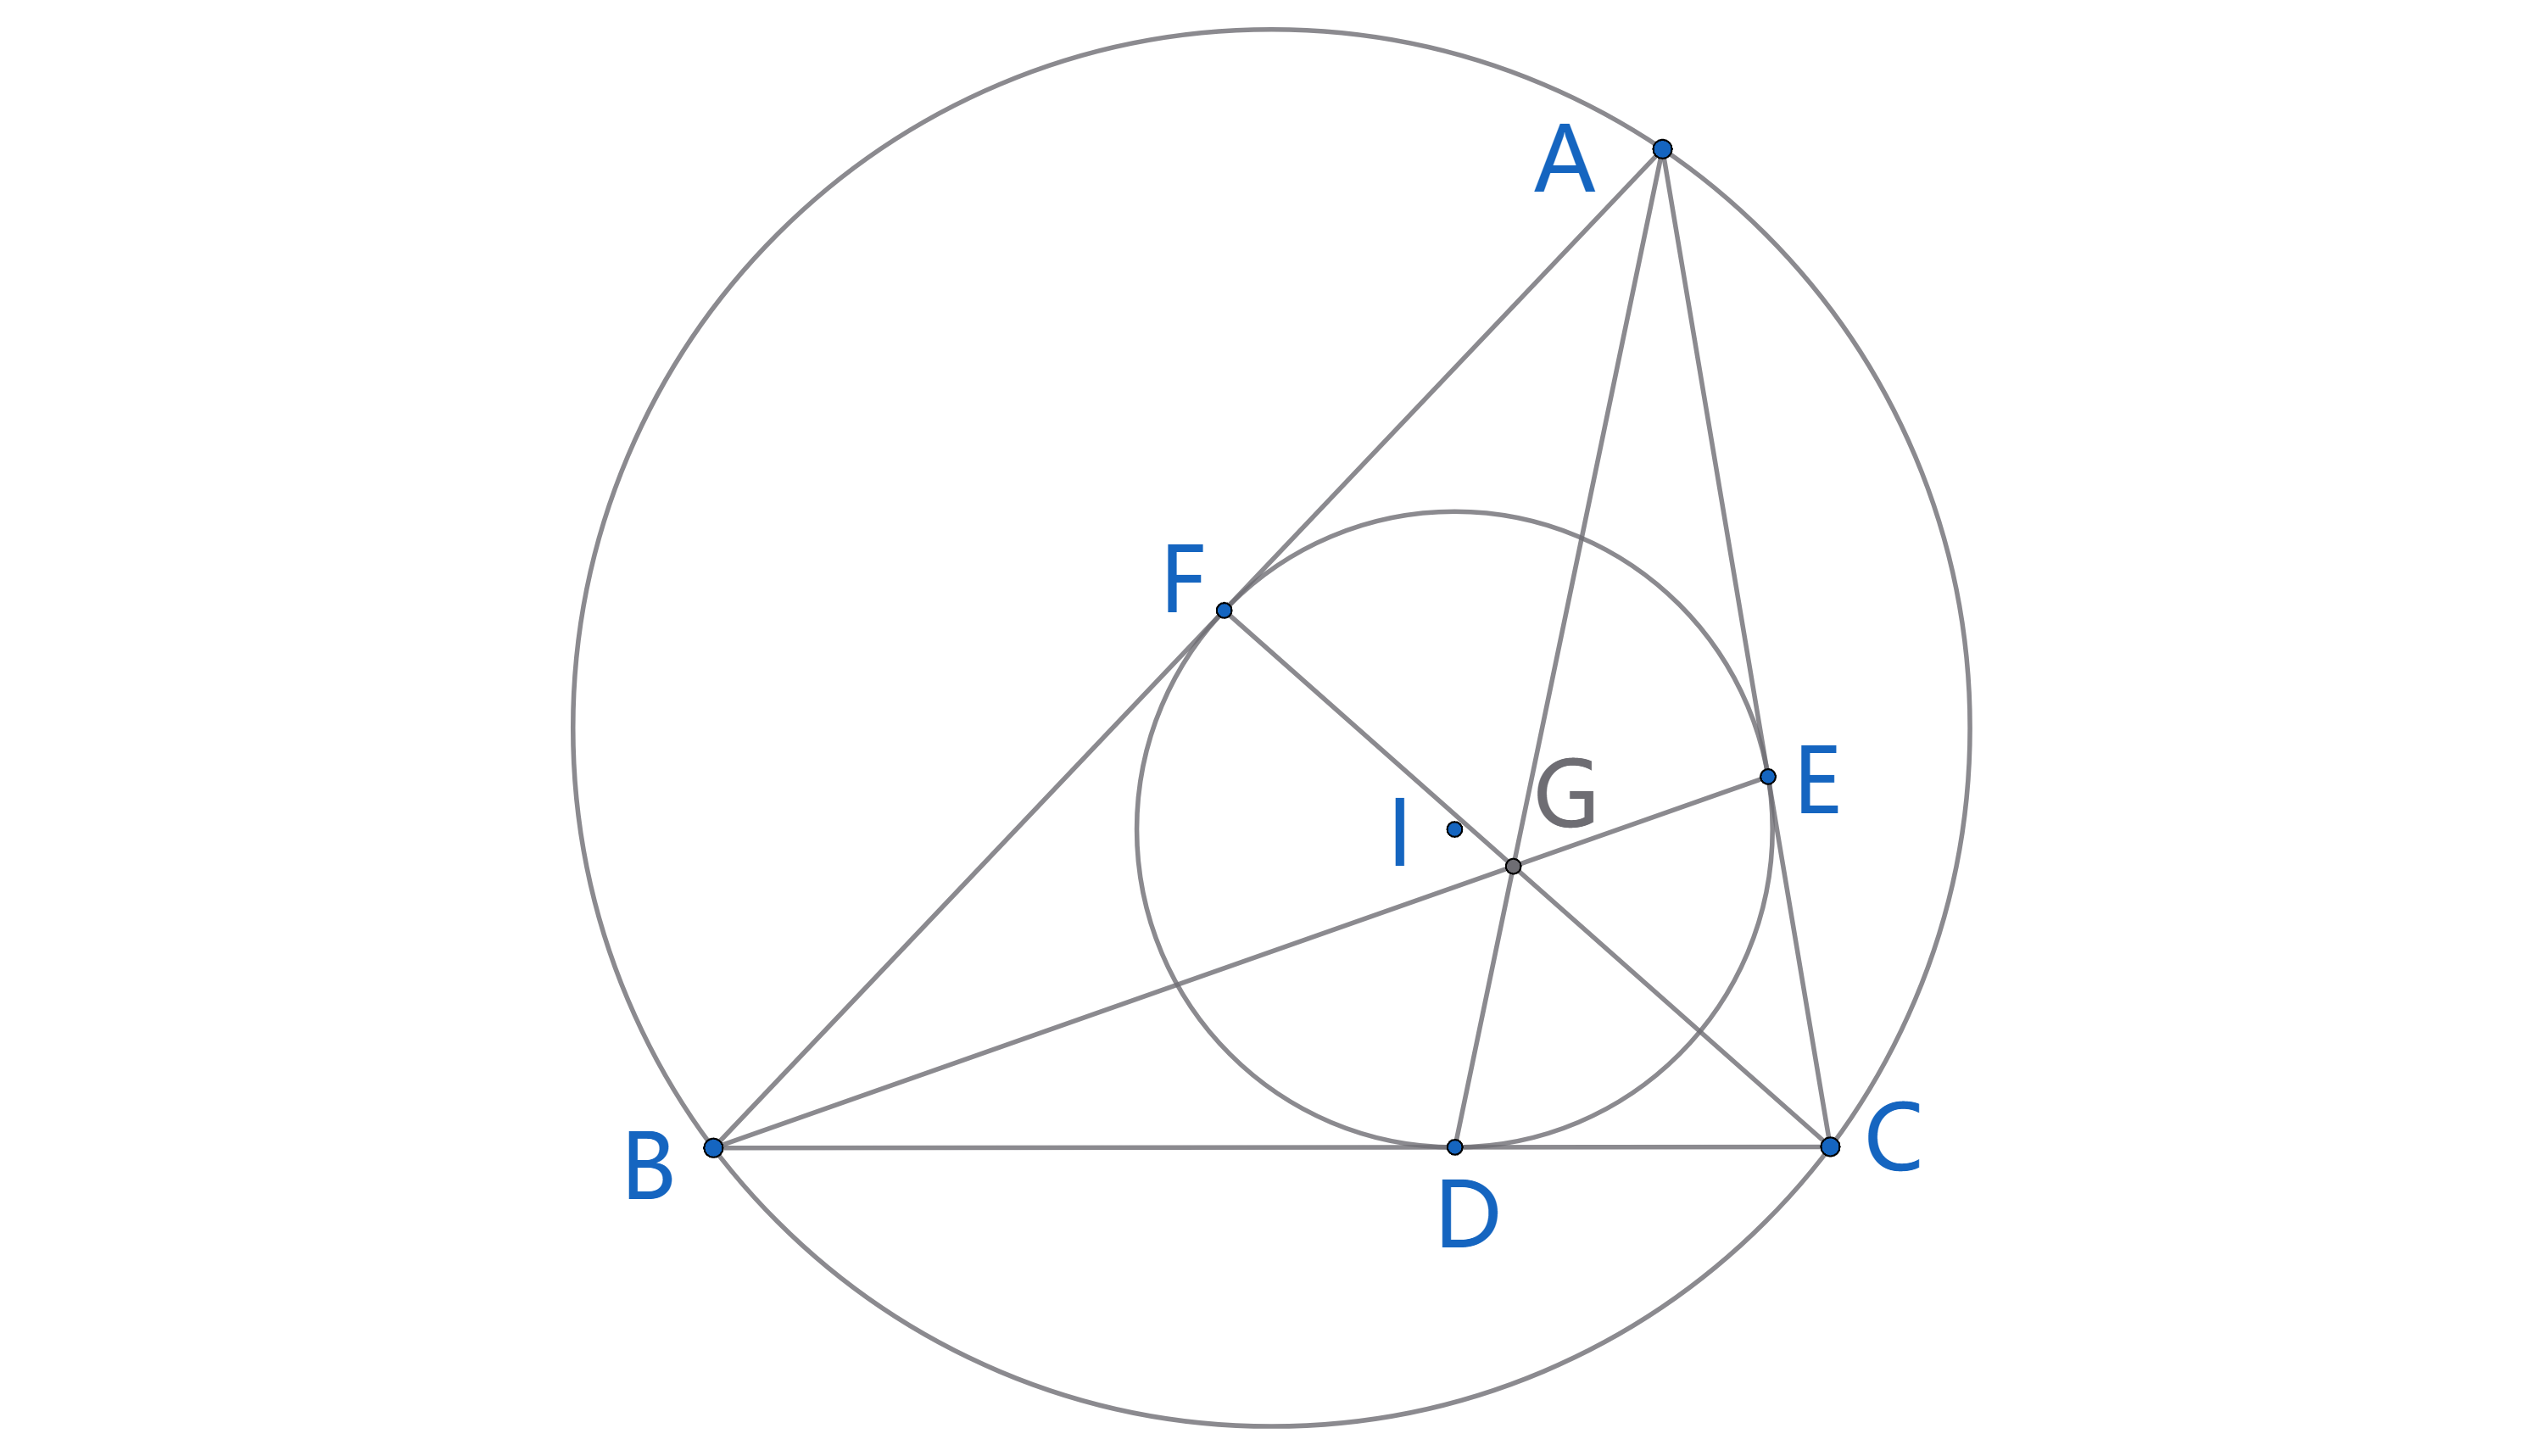
\includegraphics[width=0.7\linewidth]{figures/exercises/316.png}
\end{figure}


\begin{exercise}
在圆内接四边形 $ABCD$ 中,点 $X$ 和 $Y$ 分别是 $\triangle ABC$ 和 $\triangle BCD$ 的垂心。证明:$AXYD$ 是平行四边形。
\end{exercise}
\begin{figure}[H]
    \centering
    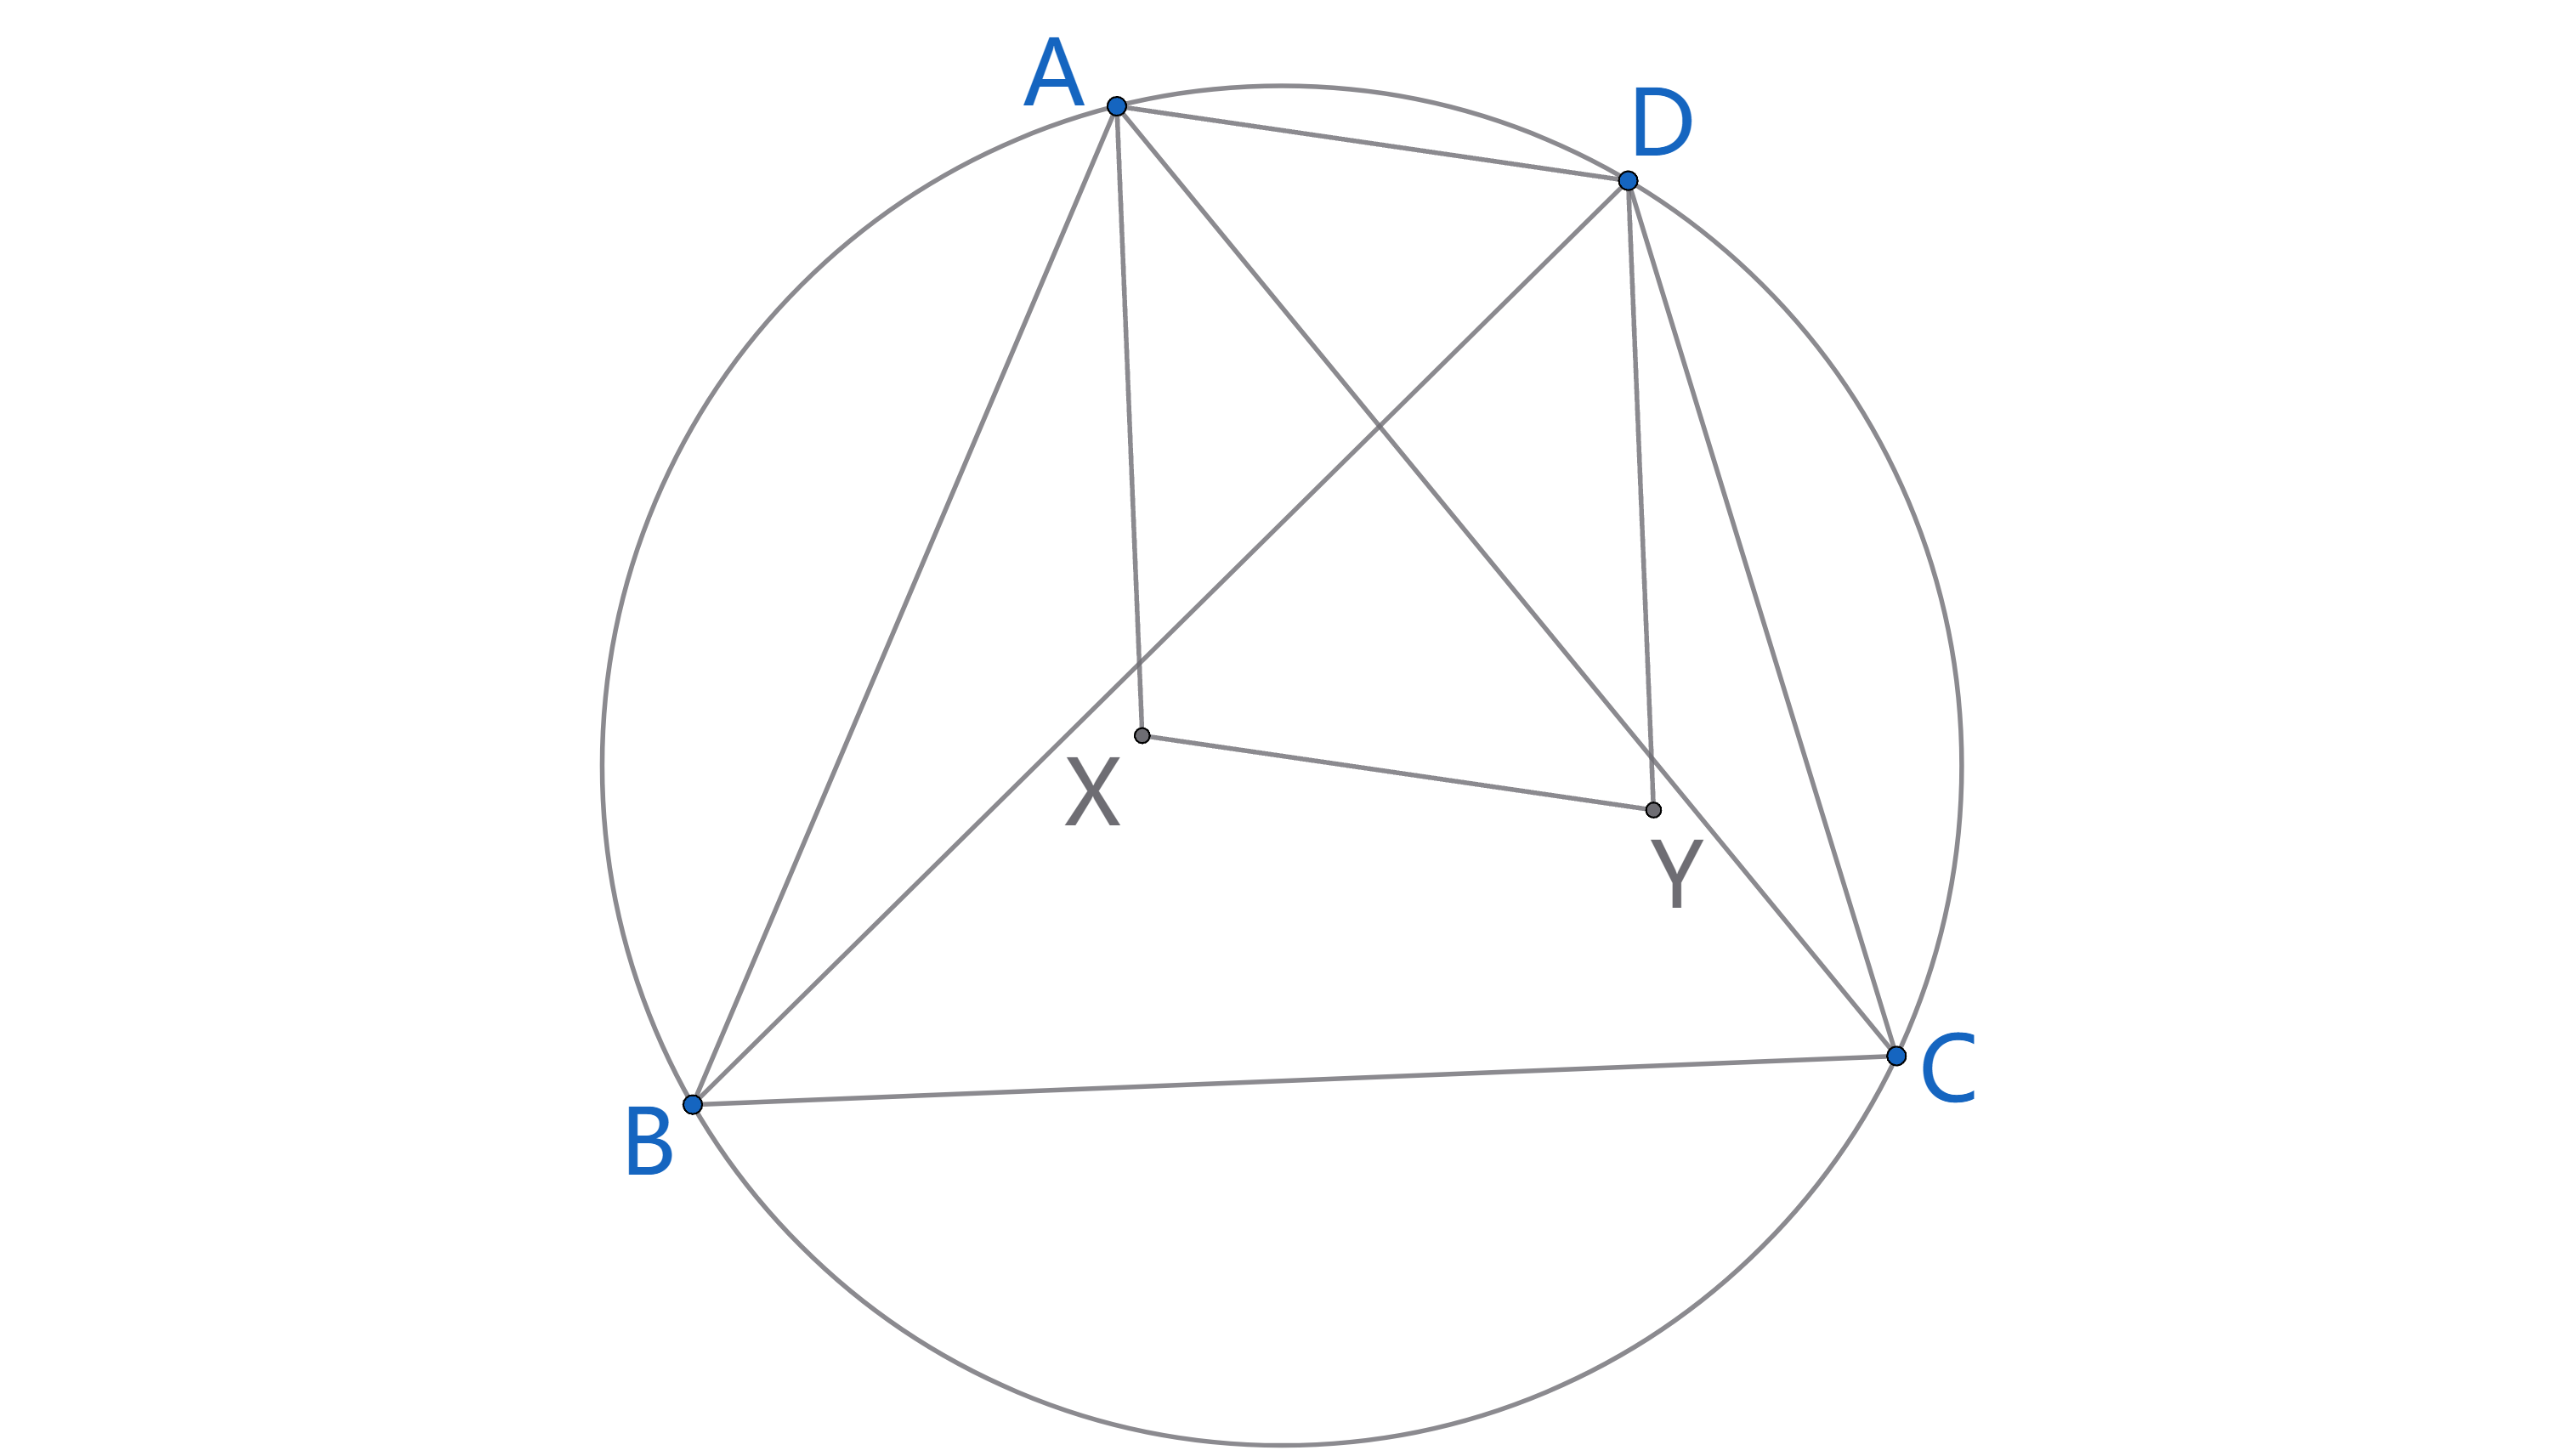
\includegraphics[width=0.7\linewidth]{figures/exercises/317.png}
\end{figure}


%-----------------------------------
\newpage 
\begin{exercise}
    设 $AD, BE, CF$ 是三角形中的塞瓦线,交于一点 $P$。证明:
    $$
    \frac{PD}{AD} + \frac{PE}{BE} + \frac{PF}{CF} = 1.
    $$
\end{exercise}
\begin{figure}[H]
    \centering
    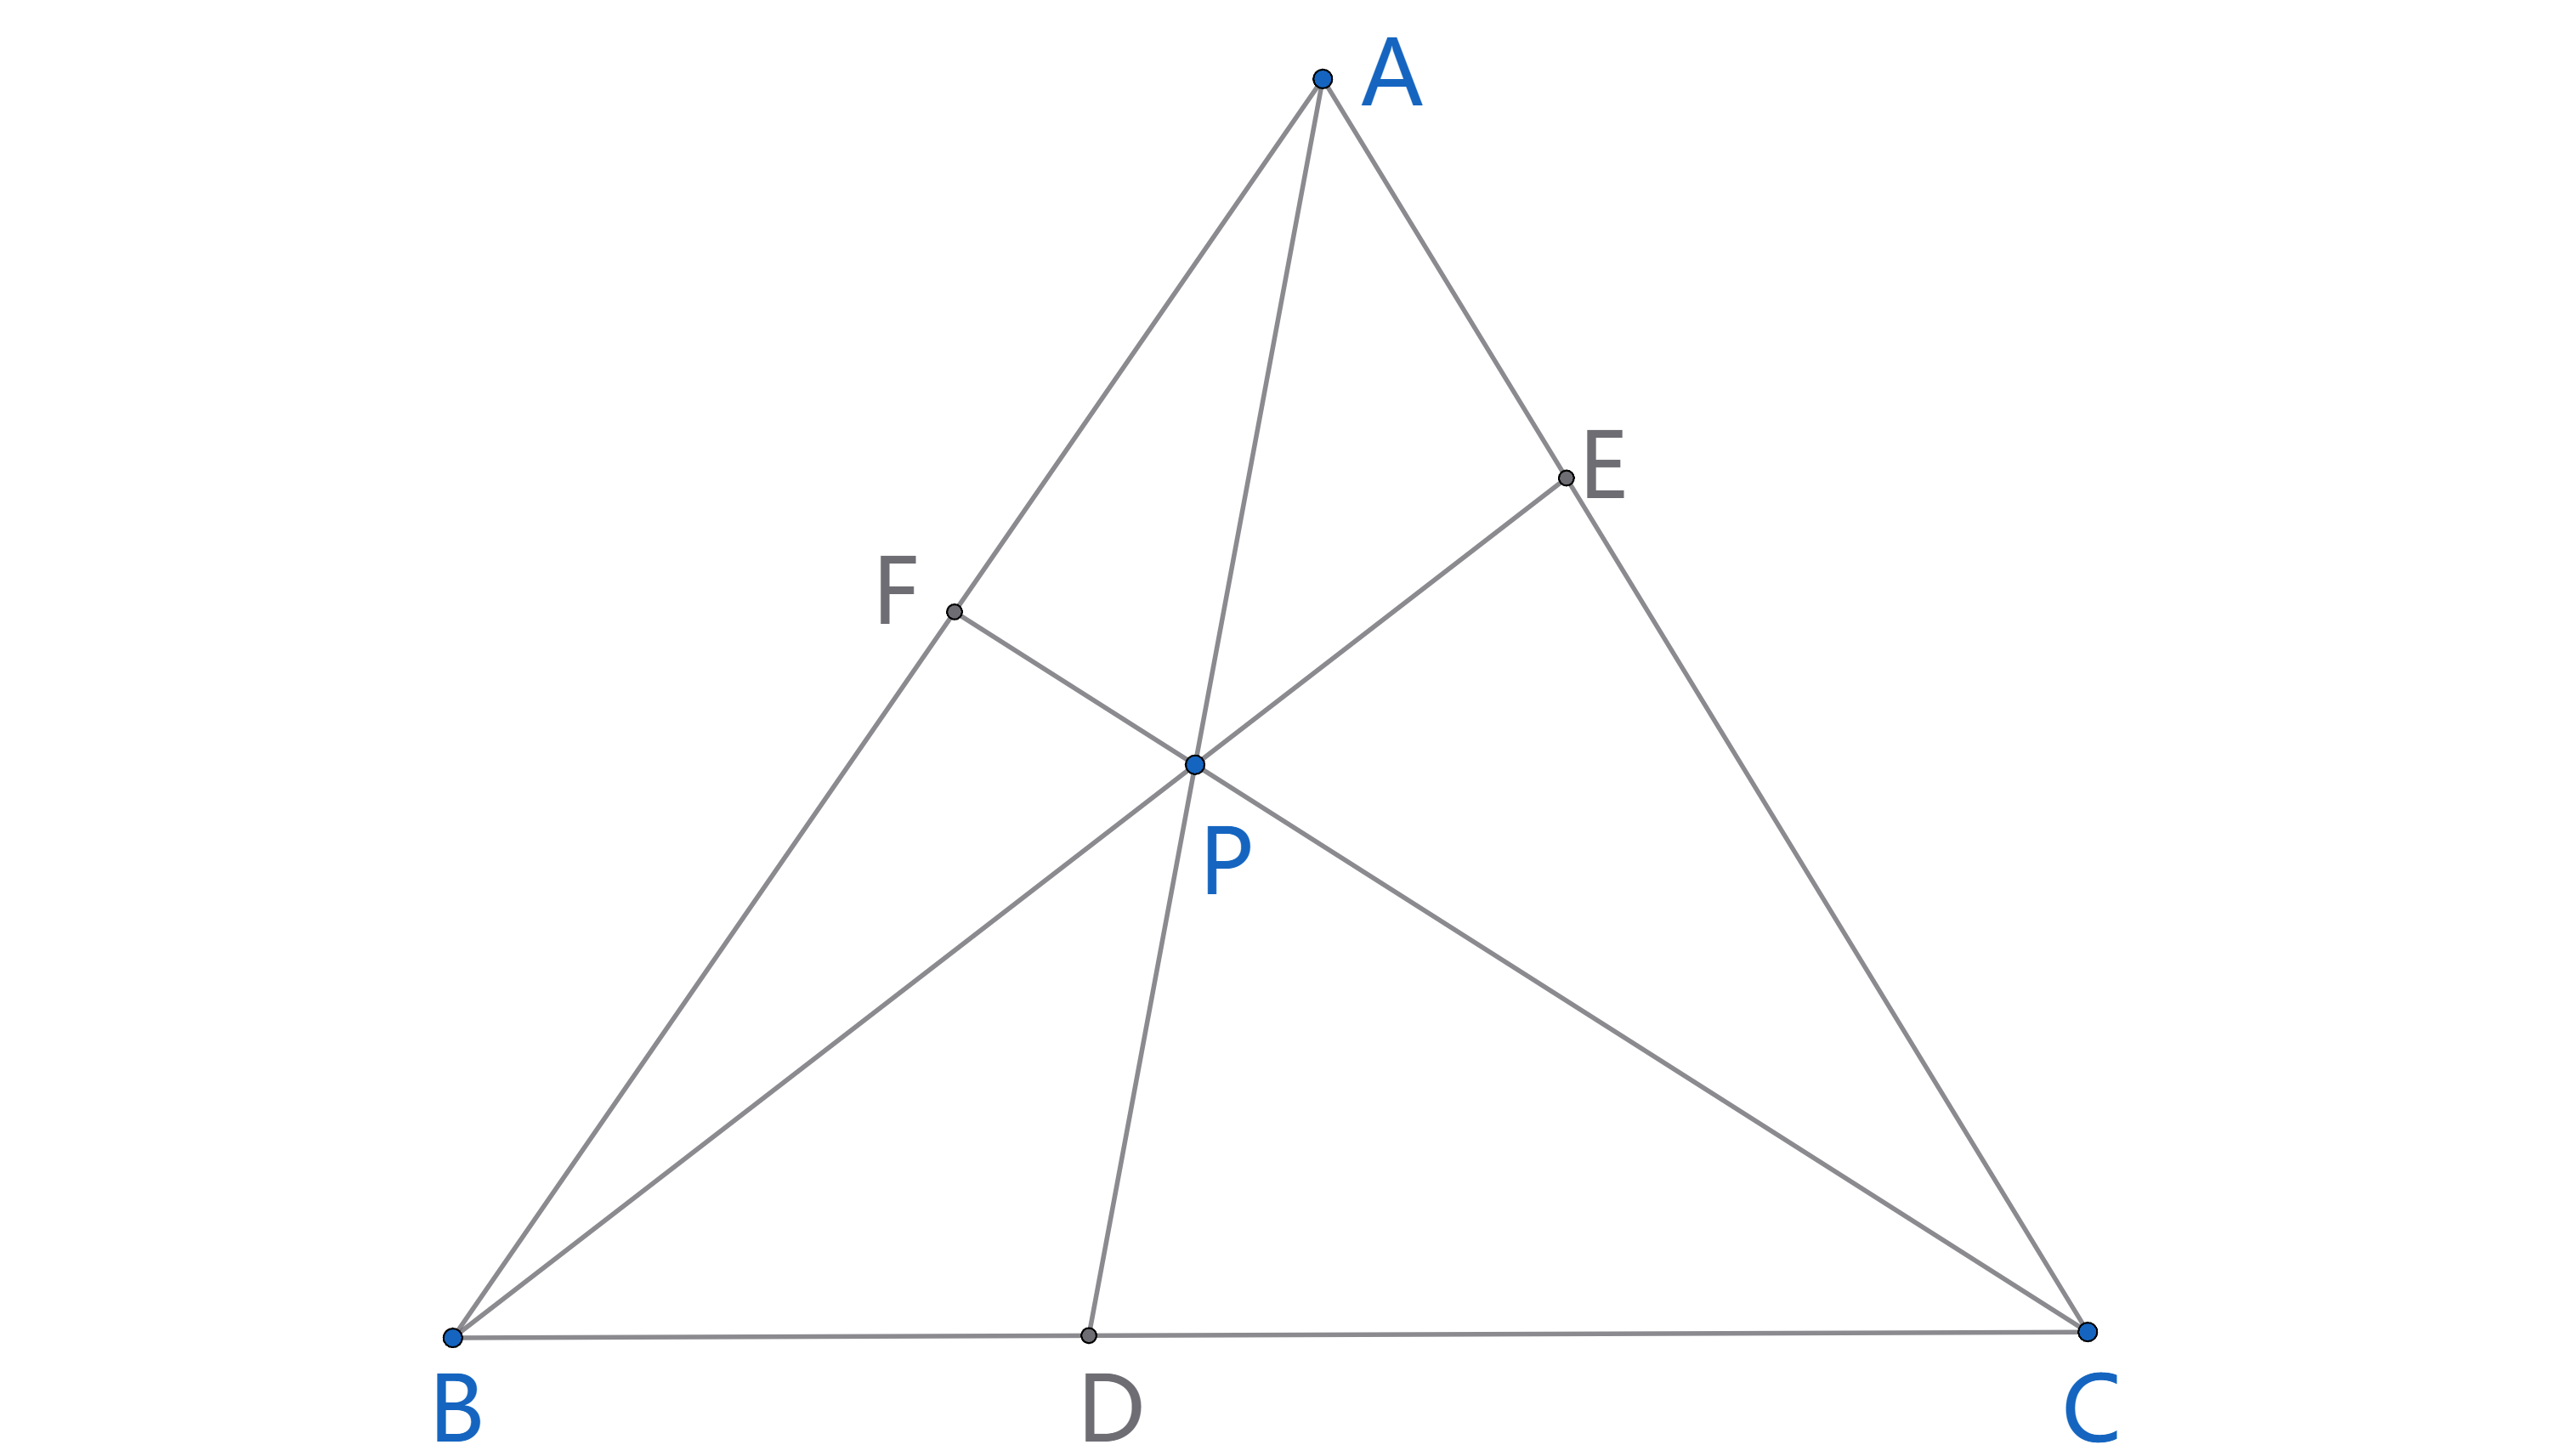
\includegraphics[width=0.7\linewidth]{figures/exercises/318.png}
\end{figure}

\begin{exercise}
(预选题 2006/G3) 设凸五边形 $ABCDE$ 满足 $\angle BAC = \angle CAD = \angle DAE, \angle ABC = \angle ACD = \angle ADE$。对角线 $BD$ 和 $CE$ 交于点 $P$。证明:射线 $AP$ 平分 ${CD}$。
\end{exercise}
\begin{figure}[H]
    \centering
    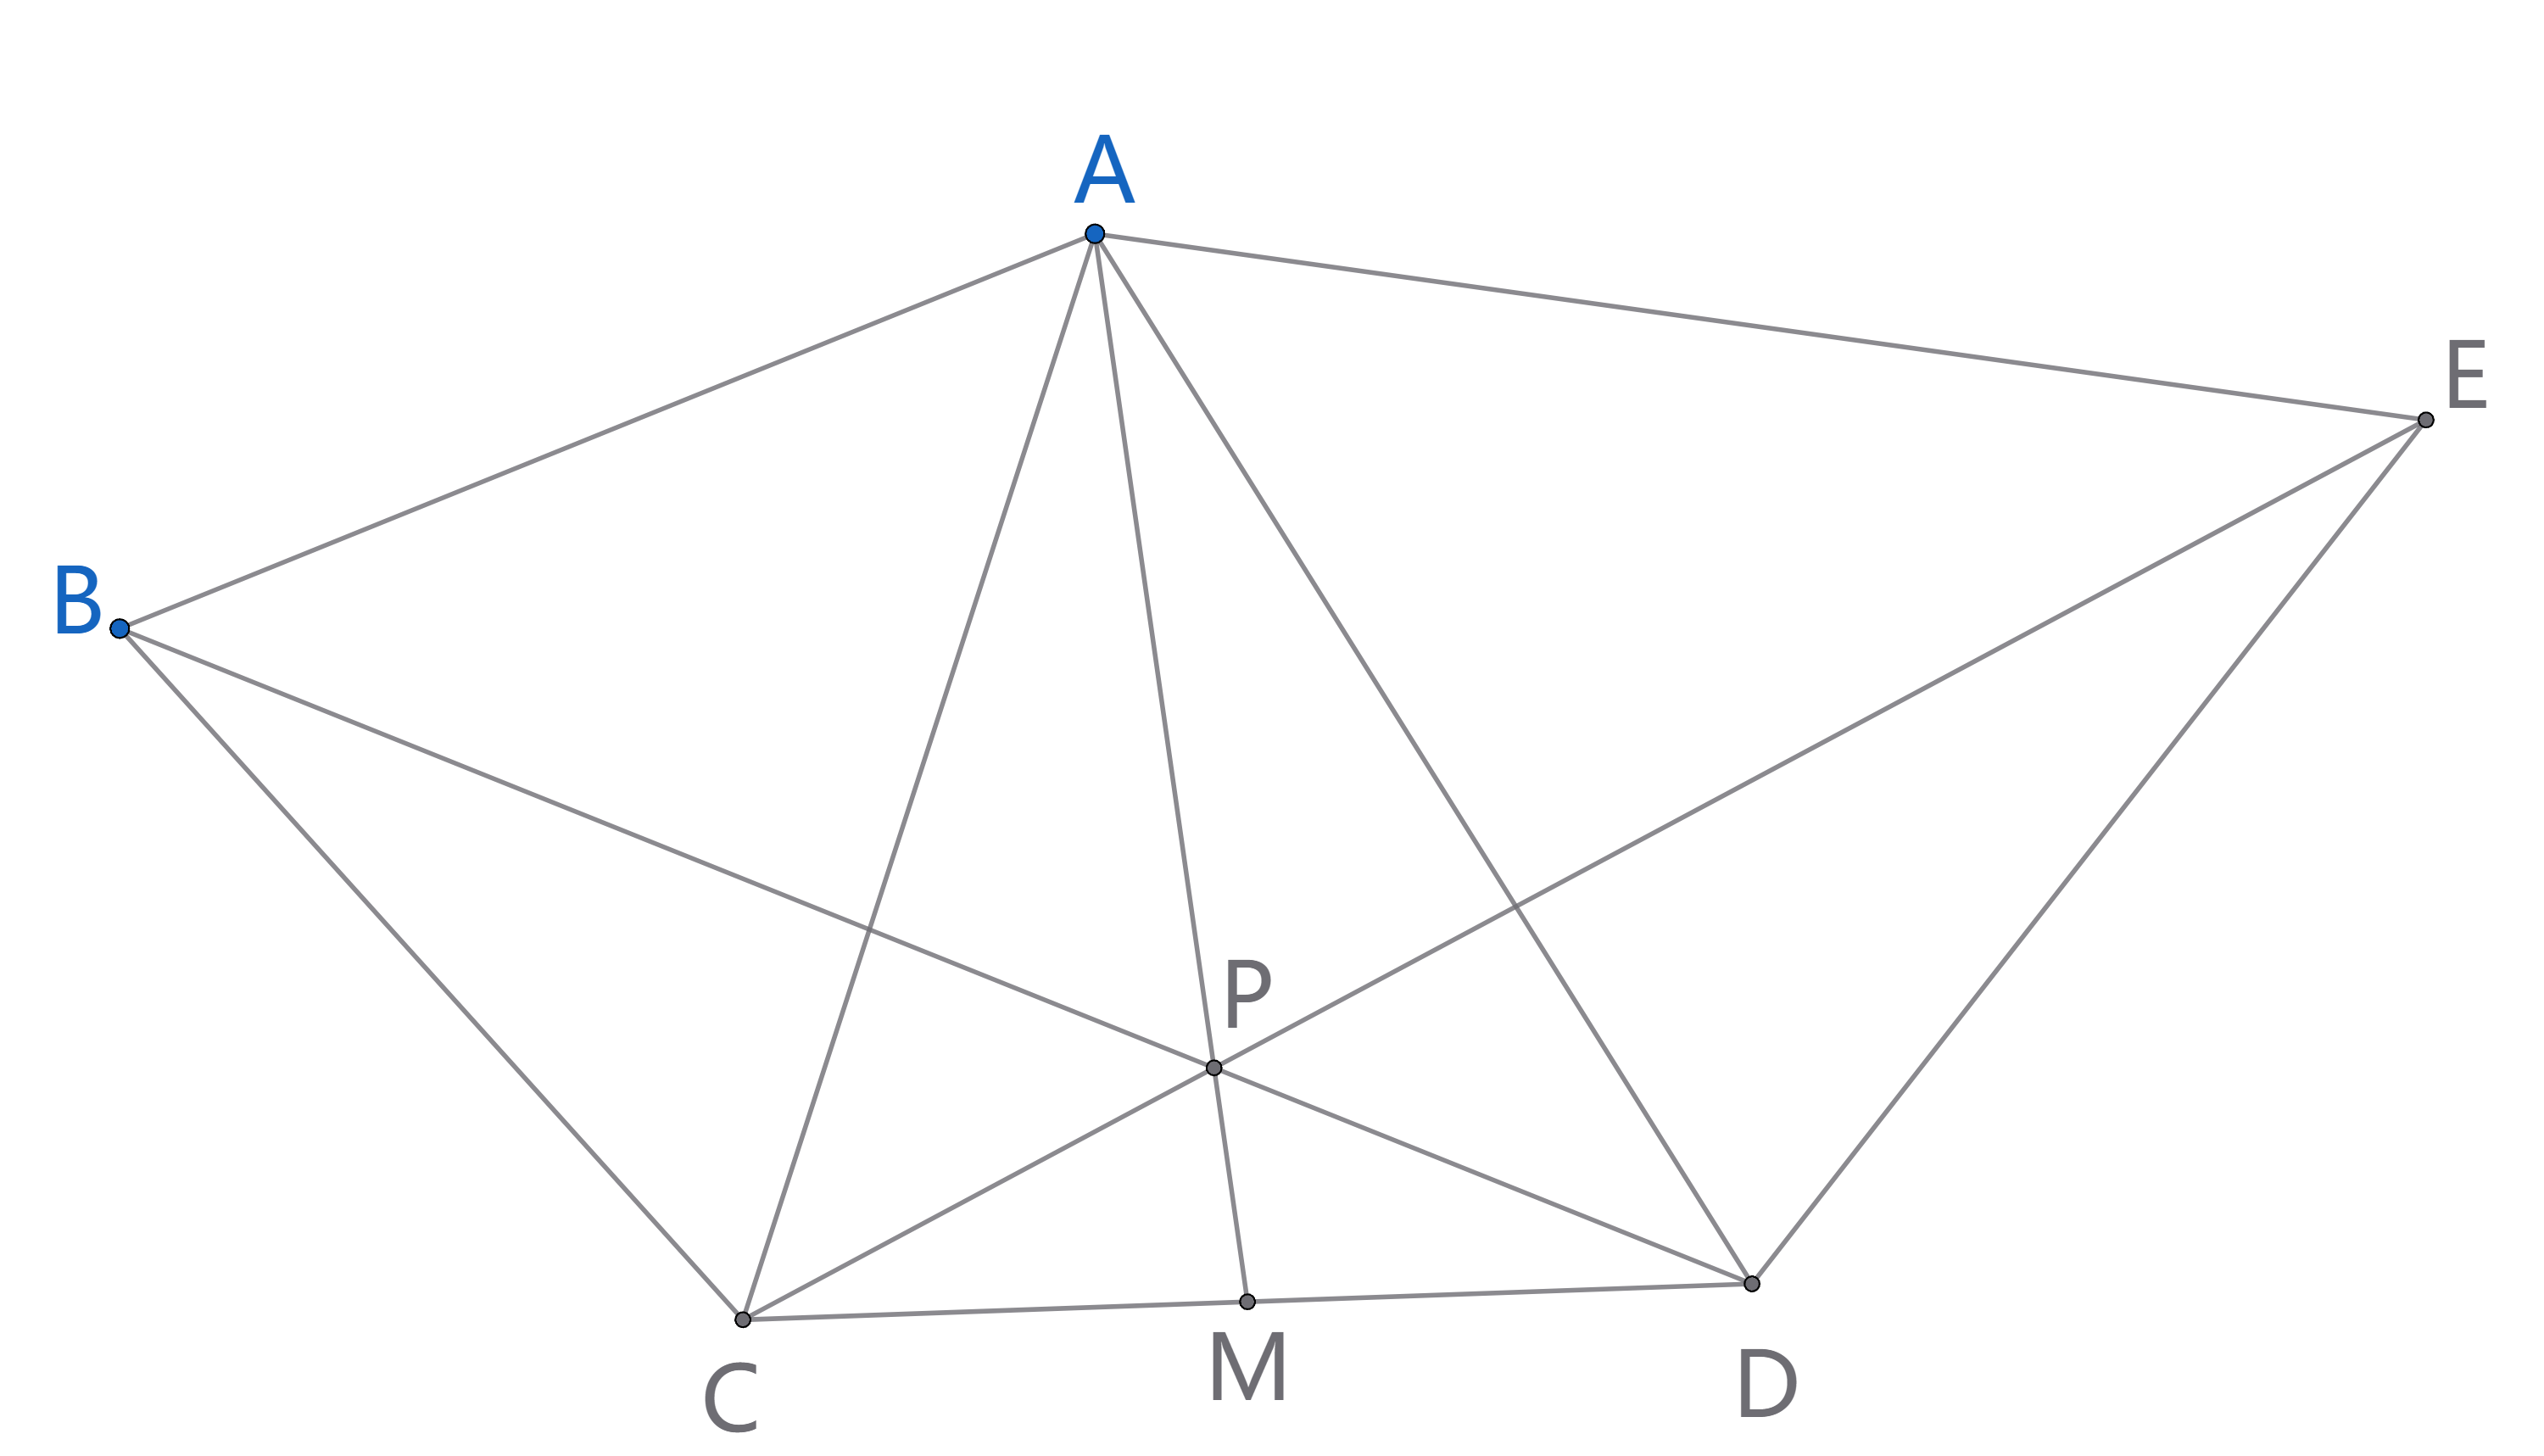
\includegraphics[width=0.7\linewidth]{figures/exercises/319.png}
\end{figure}


%-----------------------------------
\newpage 
\begin{exercise}
    (BAMO 2013/3) 设 $H$ 是锐角 $\triangle ABC$ 的垂心,考虑 $\triangle ABH, \triangle BCH, \triangle CAH$ 的外心。证明:这三个外心构成的三角形与 $\triangle ABC$ 全等。
\end{exercise}
\begin{figure}[H]
    \centering
    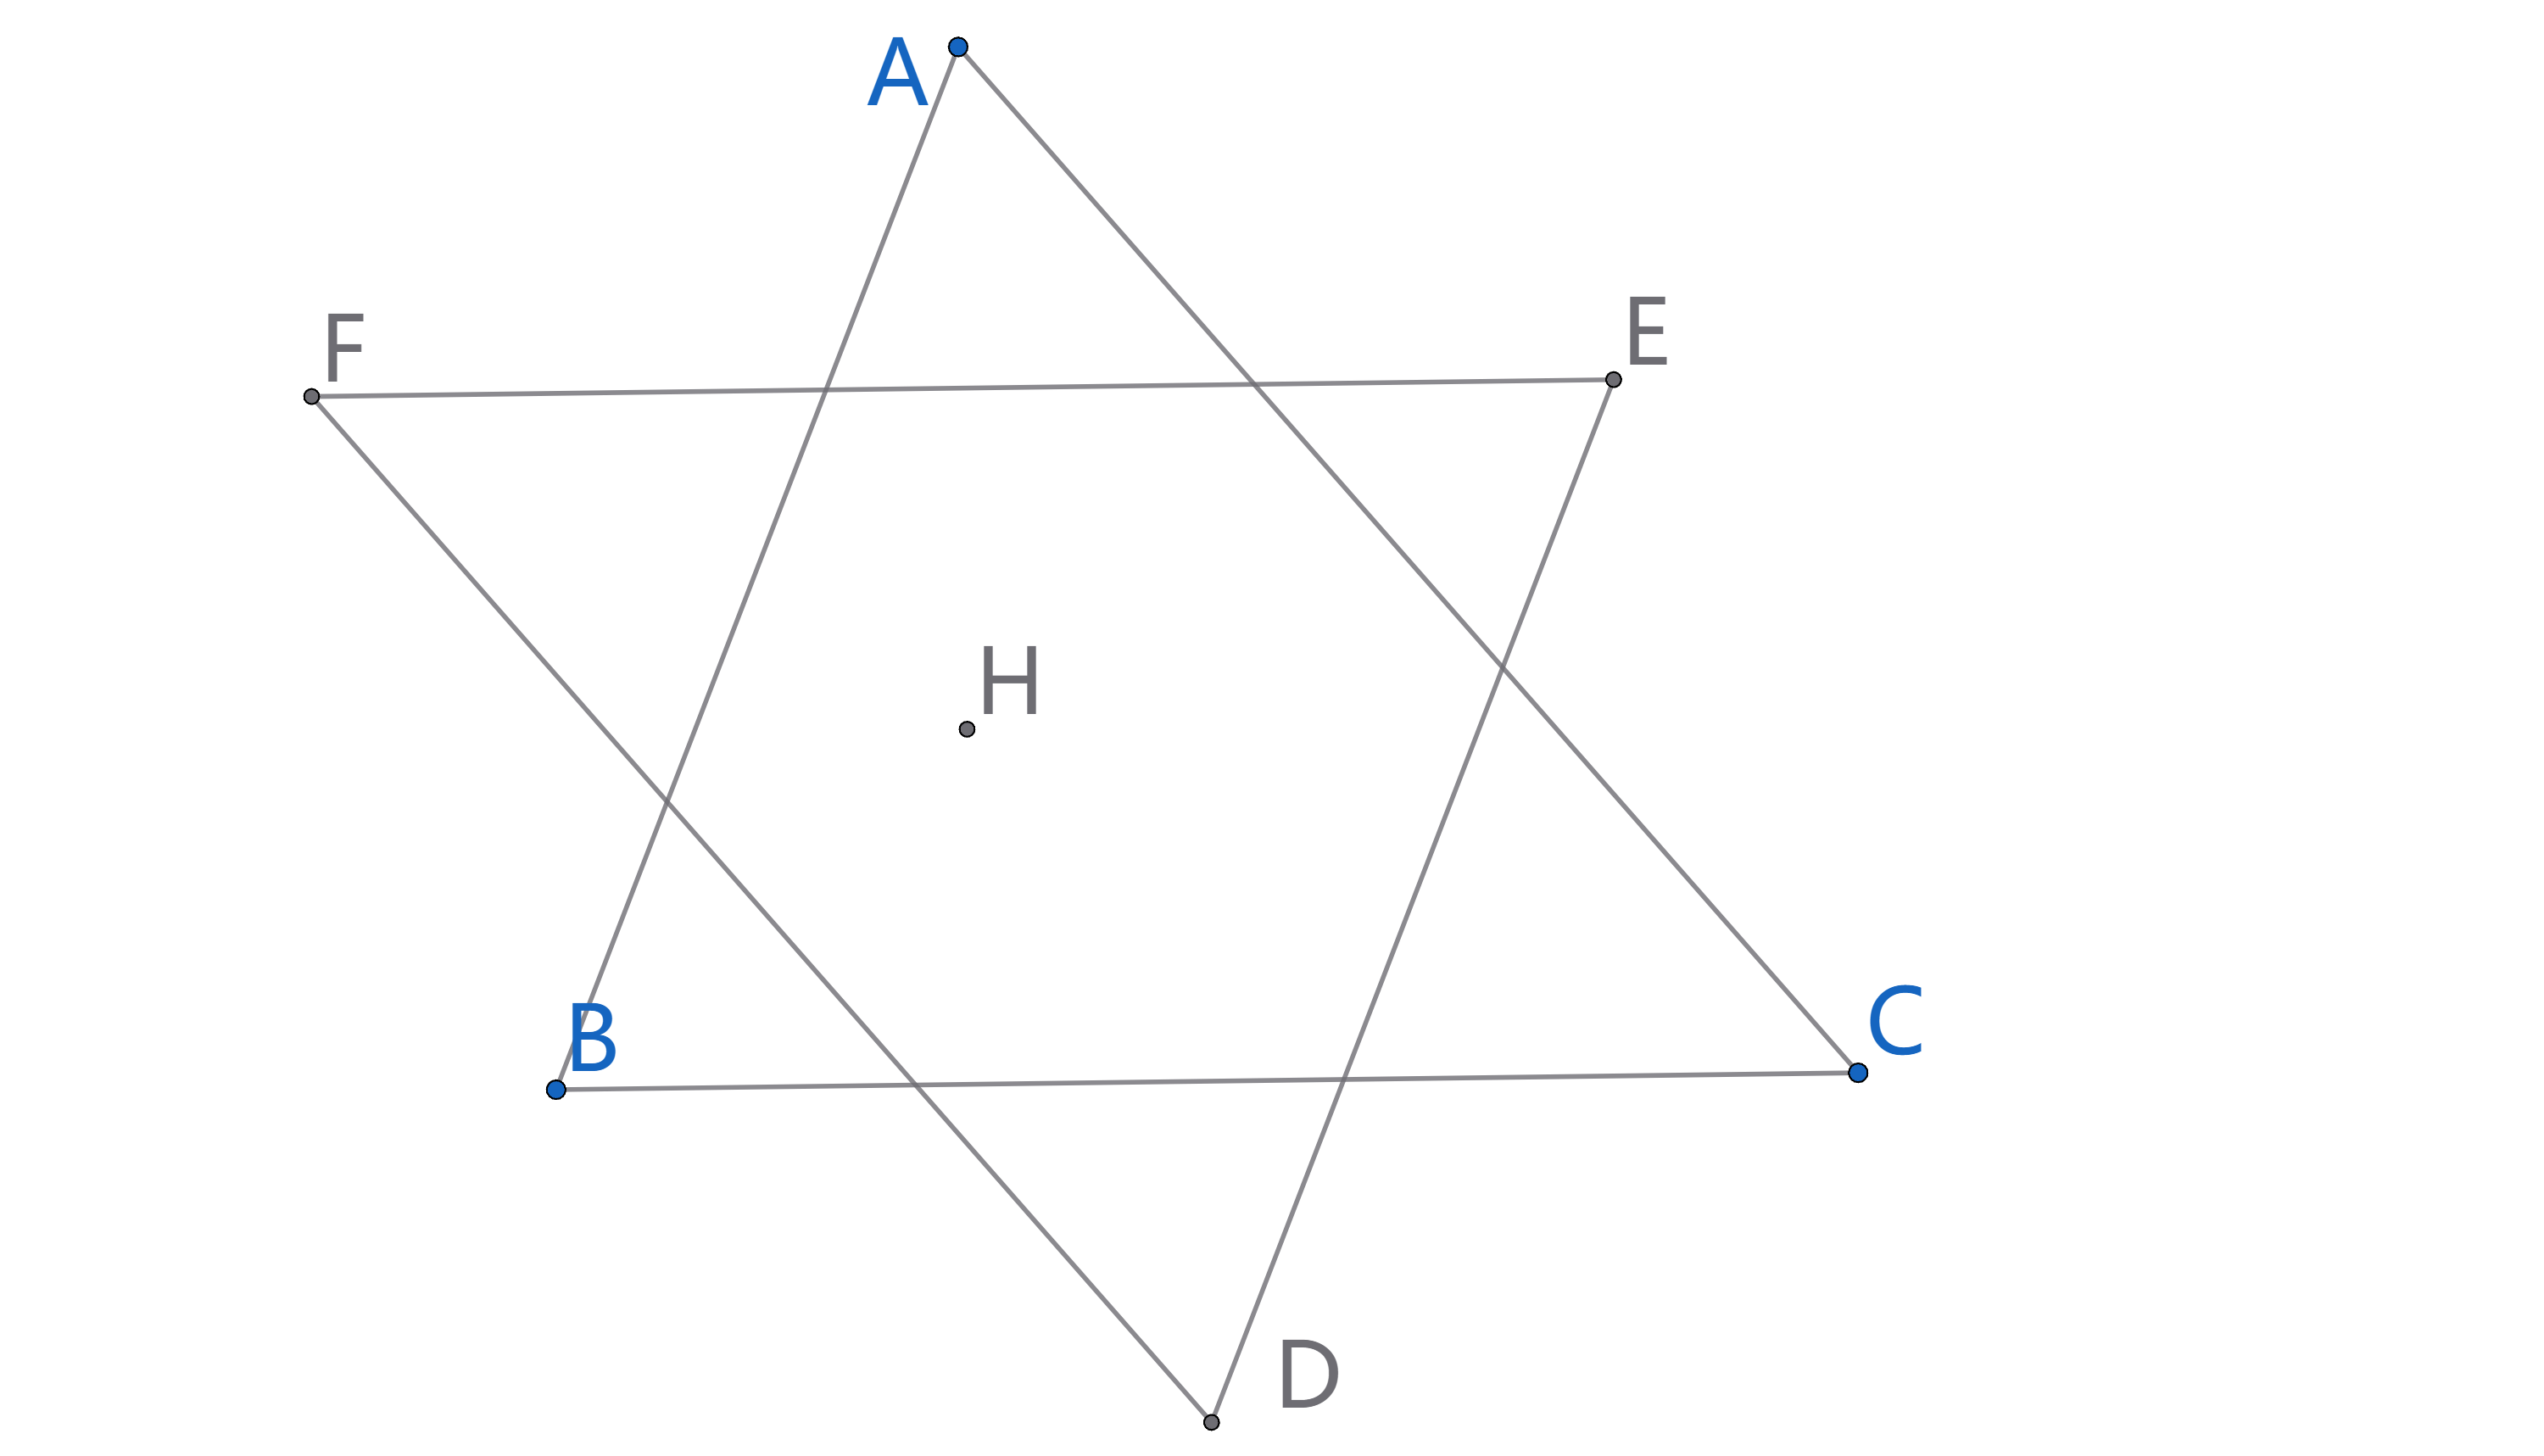
\includegraphics[width=0.7\linewidth]{figures/exercises/320.png}
\end{figure}

\begin{exercise}
    (USAMO 2003/4) 设 $\triangle ABC$ 中,经过点 $A, B$ 的一个圆与线段 $AC, BC$ 分别相交于 $D, E$,直线 $AB$ 与 $DE$ 相交于 $F$,直线 $BD$ 与 $CF$ 相交于 $M$。证明:$MF = MC$ 当且仅当 $MB \cdot MD = MC^2$。
\end{exercise}
\begin{figure}[H]
    \centering
    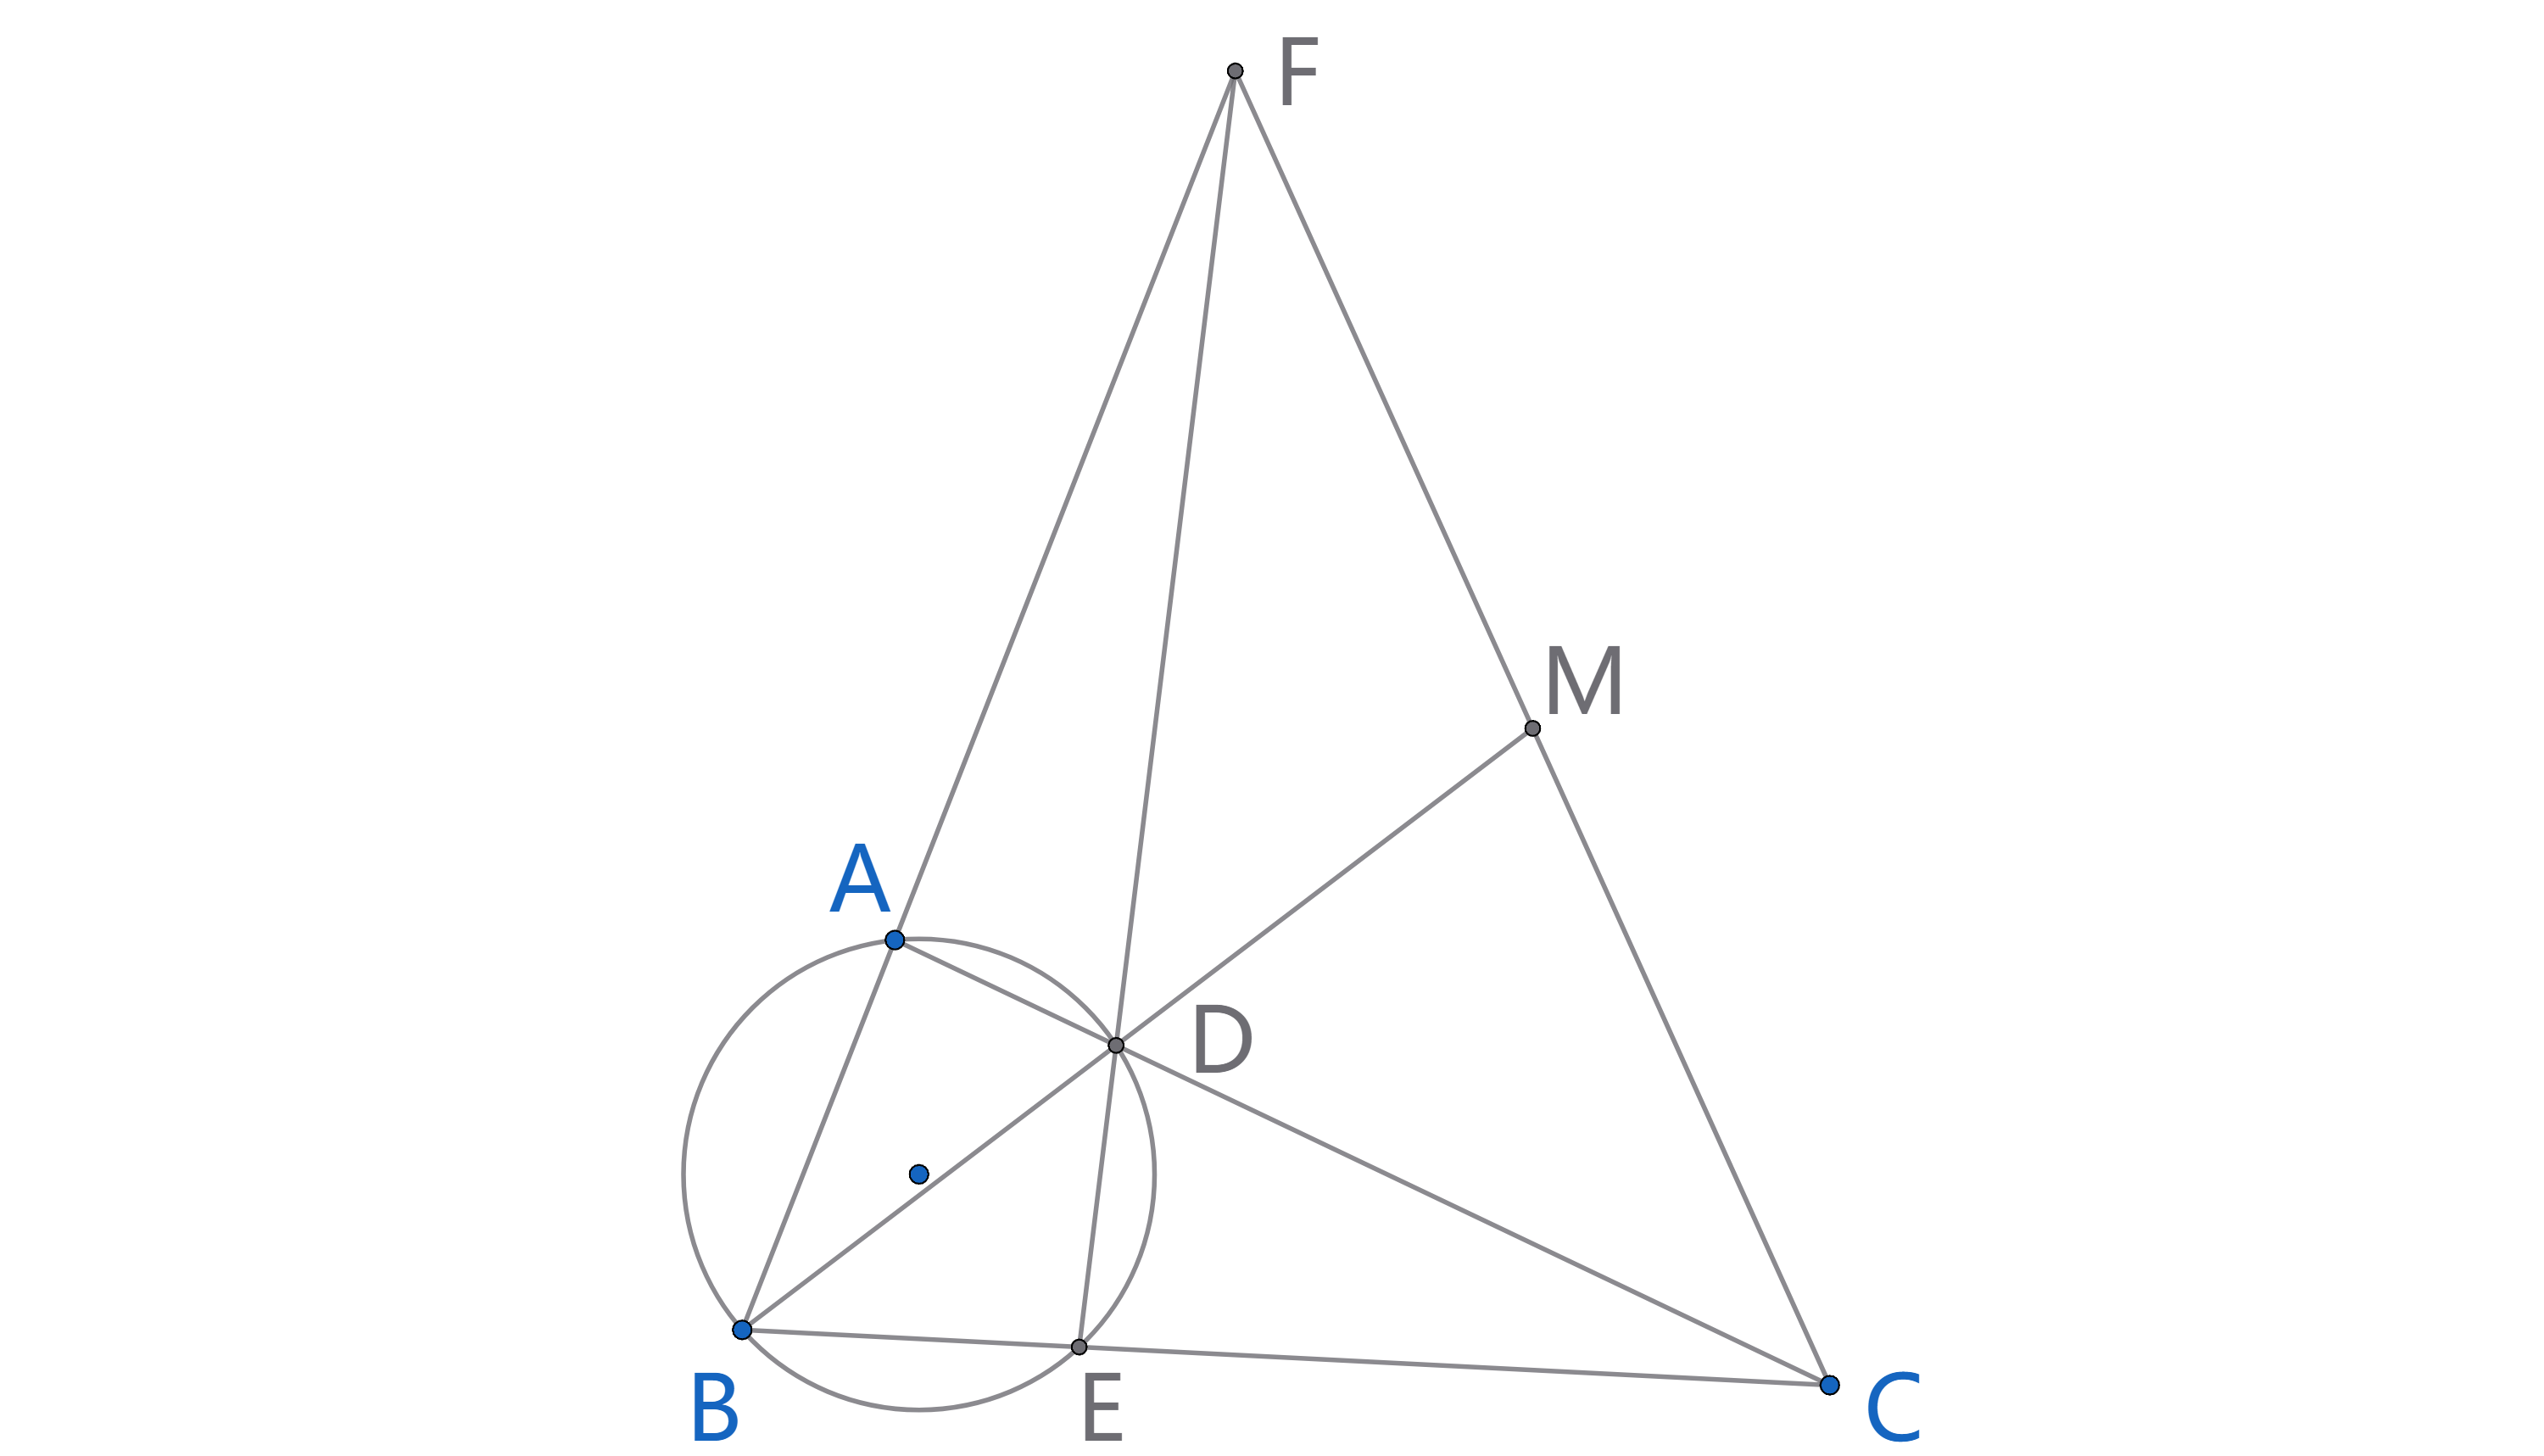
\includegraphics[width=0.7\linewidth]{figures/exercises/321.png}
\end{figure}

% \begin{exercise}
%     (蒙日定理) 如图 3.7A,考虑平面上相离的圆 $\omega_1, \omega_2, \omega_3$,半径互不相等,对每一对圆,作出它们的两条外公切线的交点,则这三个交点共线。
% \end{exercise}
% \begin{figure}[H]
%     \centering
%     \includegraphics[width=0.7\linewidth]{figures/exercises/322.png}
% \end{figure}


%-----------------------------------
\newpage 
\begin{exercise}
    设锐角 $\triangle ABC$ 的外接圆上一点 $D \neq A$,满足 $AD \parallel {BC}$。设 $G$ 是 $\triangle ABC$ 的重心,$K$ 是从点 $A$ 出发的高的垂足。证明:$K, G, D$ 共线。
\end{exercise}
\begin{figure}[H]
    \centering
    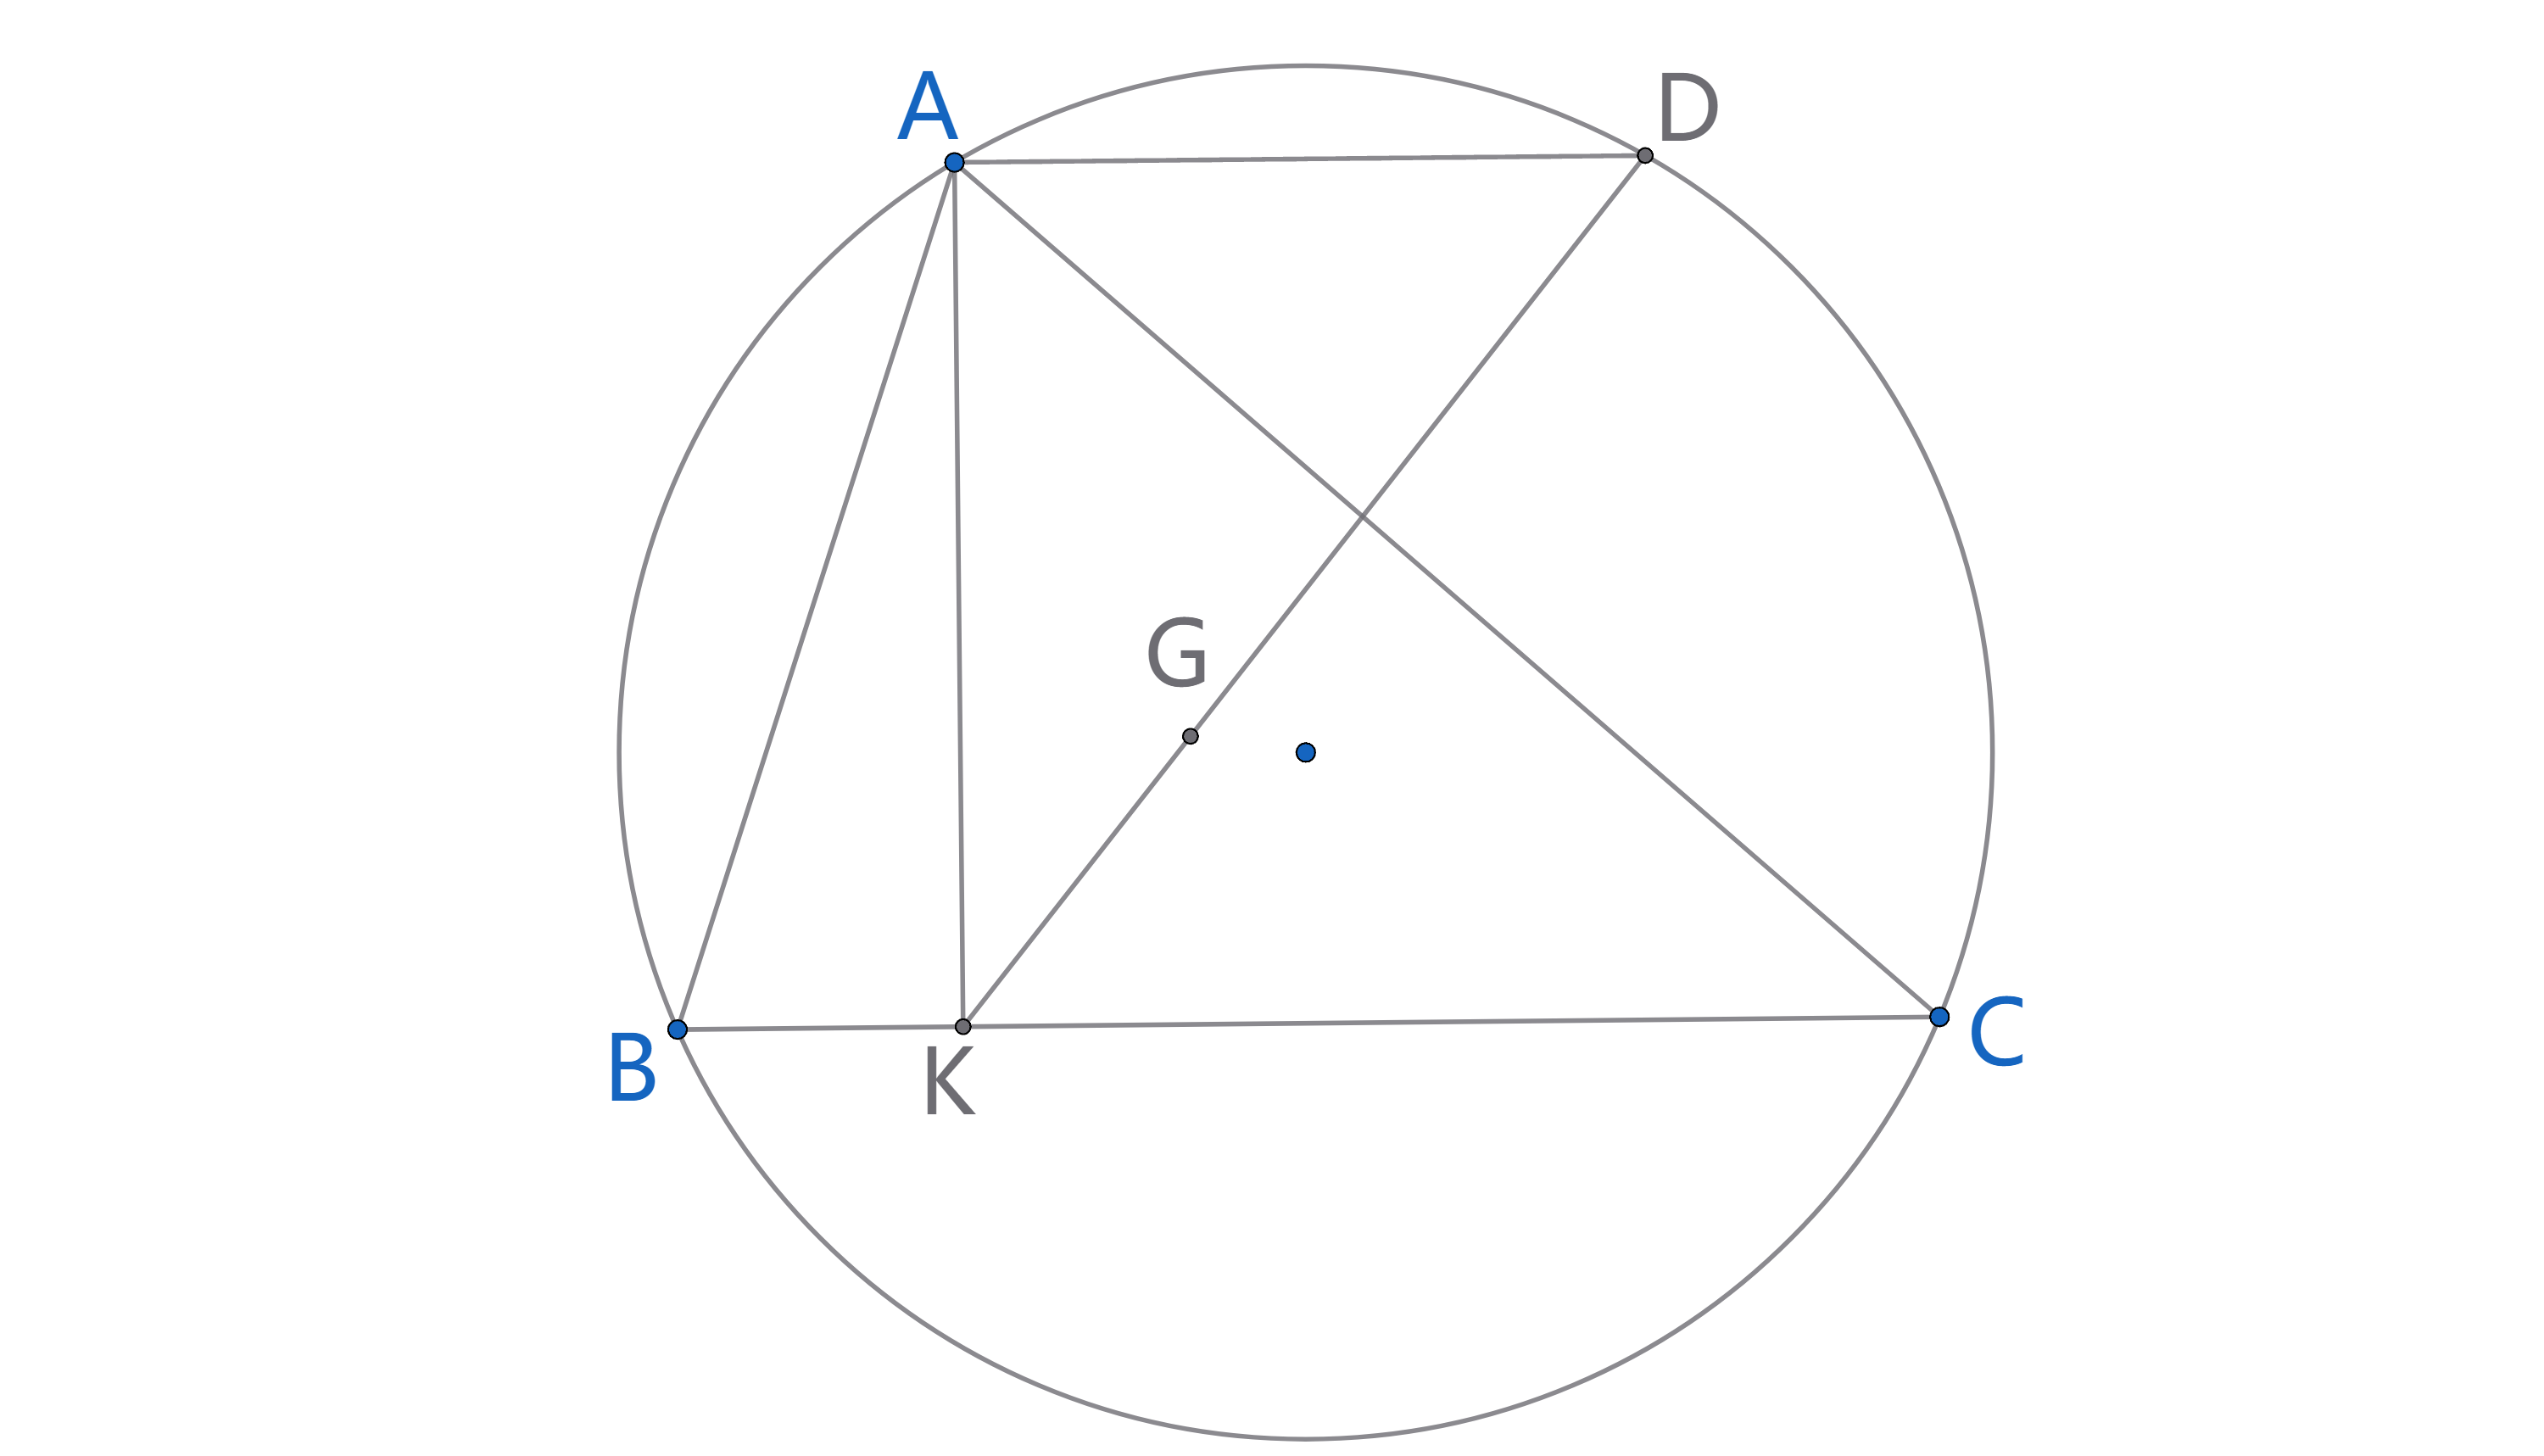
\includegraphics[width=0.7\linewidth]{figures/exercises/324.png}
\end{figure}

\begin{exercise}
    (USAMO 1993/2) 设四边形 $ABCD$ 的对角线 ${AC}, {BD}$ 垂直相交于 $E$。证明:$E$ 关于 ${AB}, {BC}, {CD}, {DA}$ 的反射点共圆。
\end{exercise}
\begin{figure}[H]
    \centering
    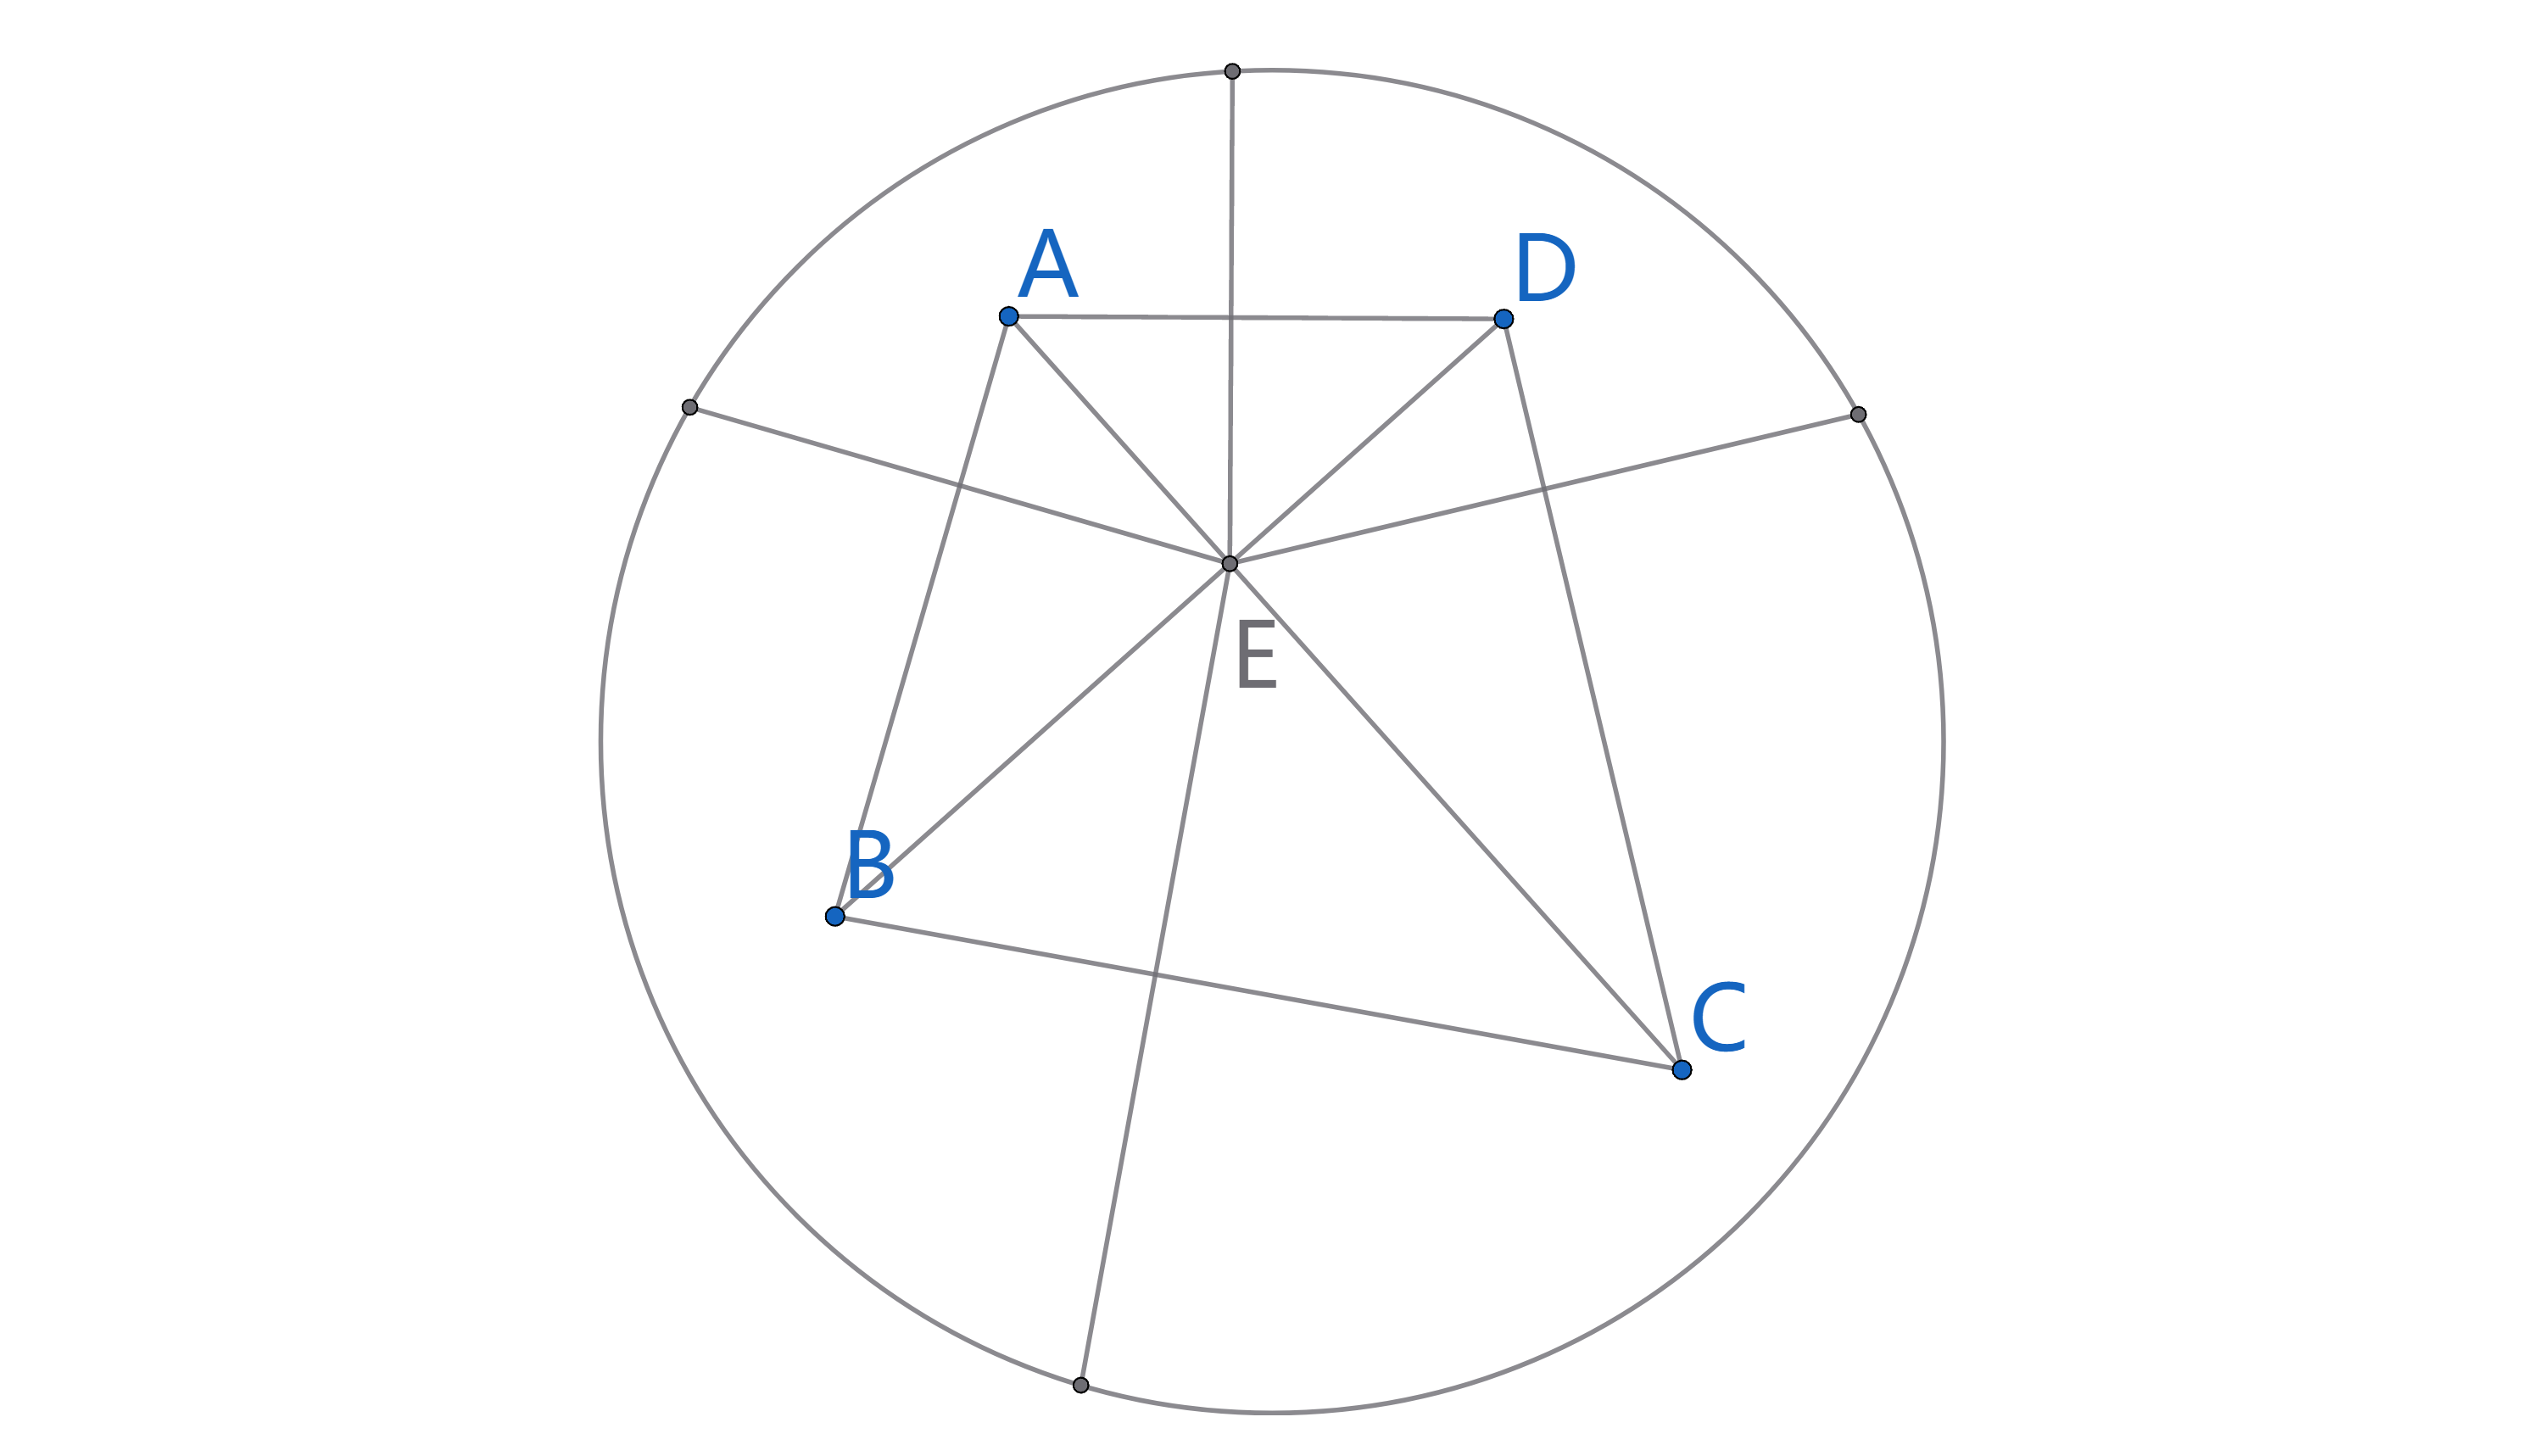
\includegraphics[width=0.7\linewidth]{figures/exercises/325.png}
\end{figure}


%-----------------------------------
\newpage 
\begin{exercise}
    (EGMO 2013/1) 将 $\triangle ABC$ 的边 ${BC}$ 延长到 $D$,使得 $CD = BC$。将边 ${CA}$ 延长到 $E$ 使得 $AE = 2CA$。证明:若 $AD = BE$,则 $\triangle ABC$ 是直角三角形。
\end{exercise}
\begin{figure}[H]
    \centering
    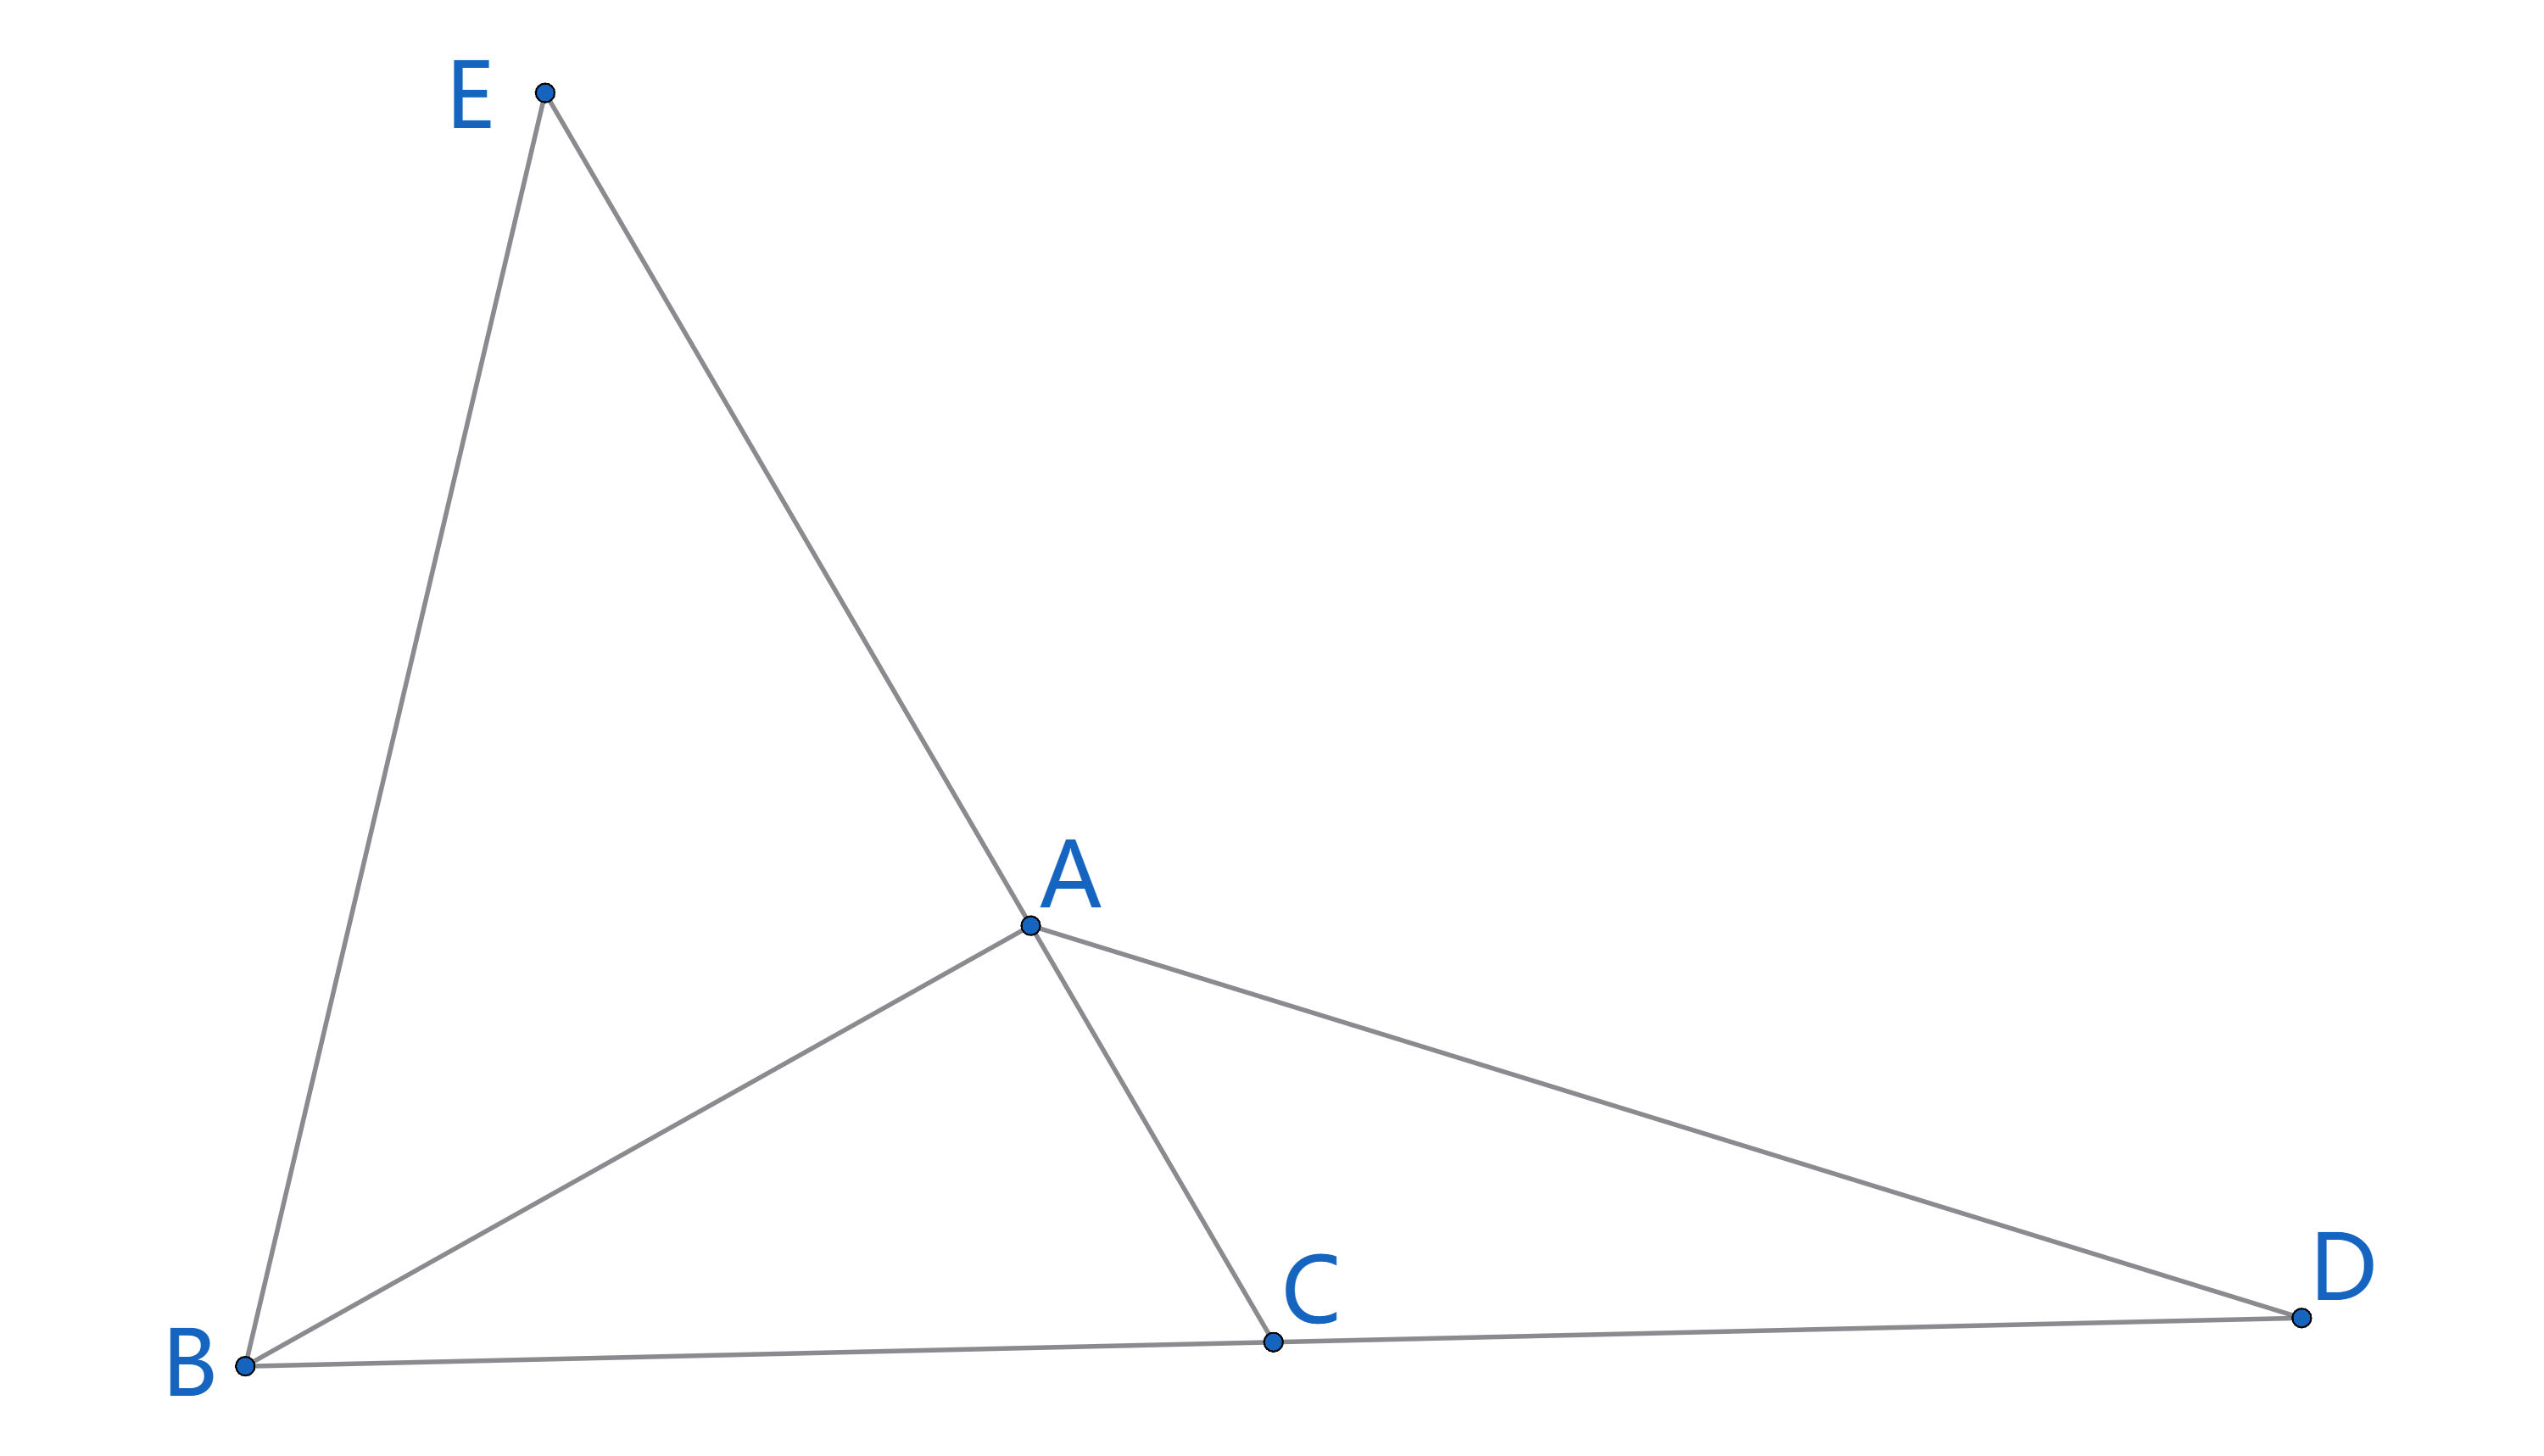
\includegraphics[width=0.7\linewidth]{figures/exercises/326.png}
\end{figure}

\begin{exercise}
    (APMO 2004/2) 设 $O$ 和 $H$ 分别是锐角 $\triangle ABC$ 的外心和垂心。证明:$\triangle AOH, \triangle BOH, \triangle COH$ 之一的面积等于另外两个面积之和。
\end{exercise}
\begin{figure}[H]
    \centering
    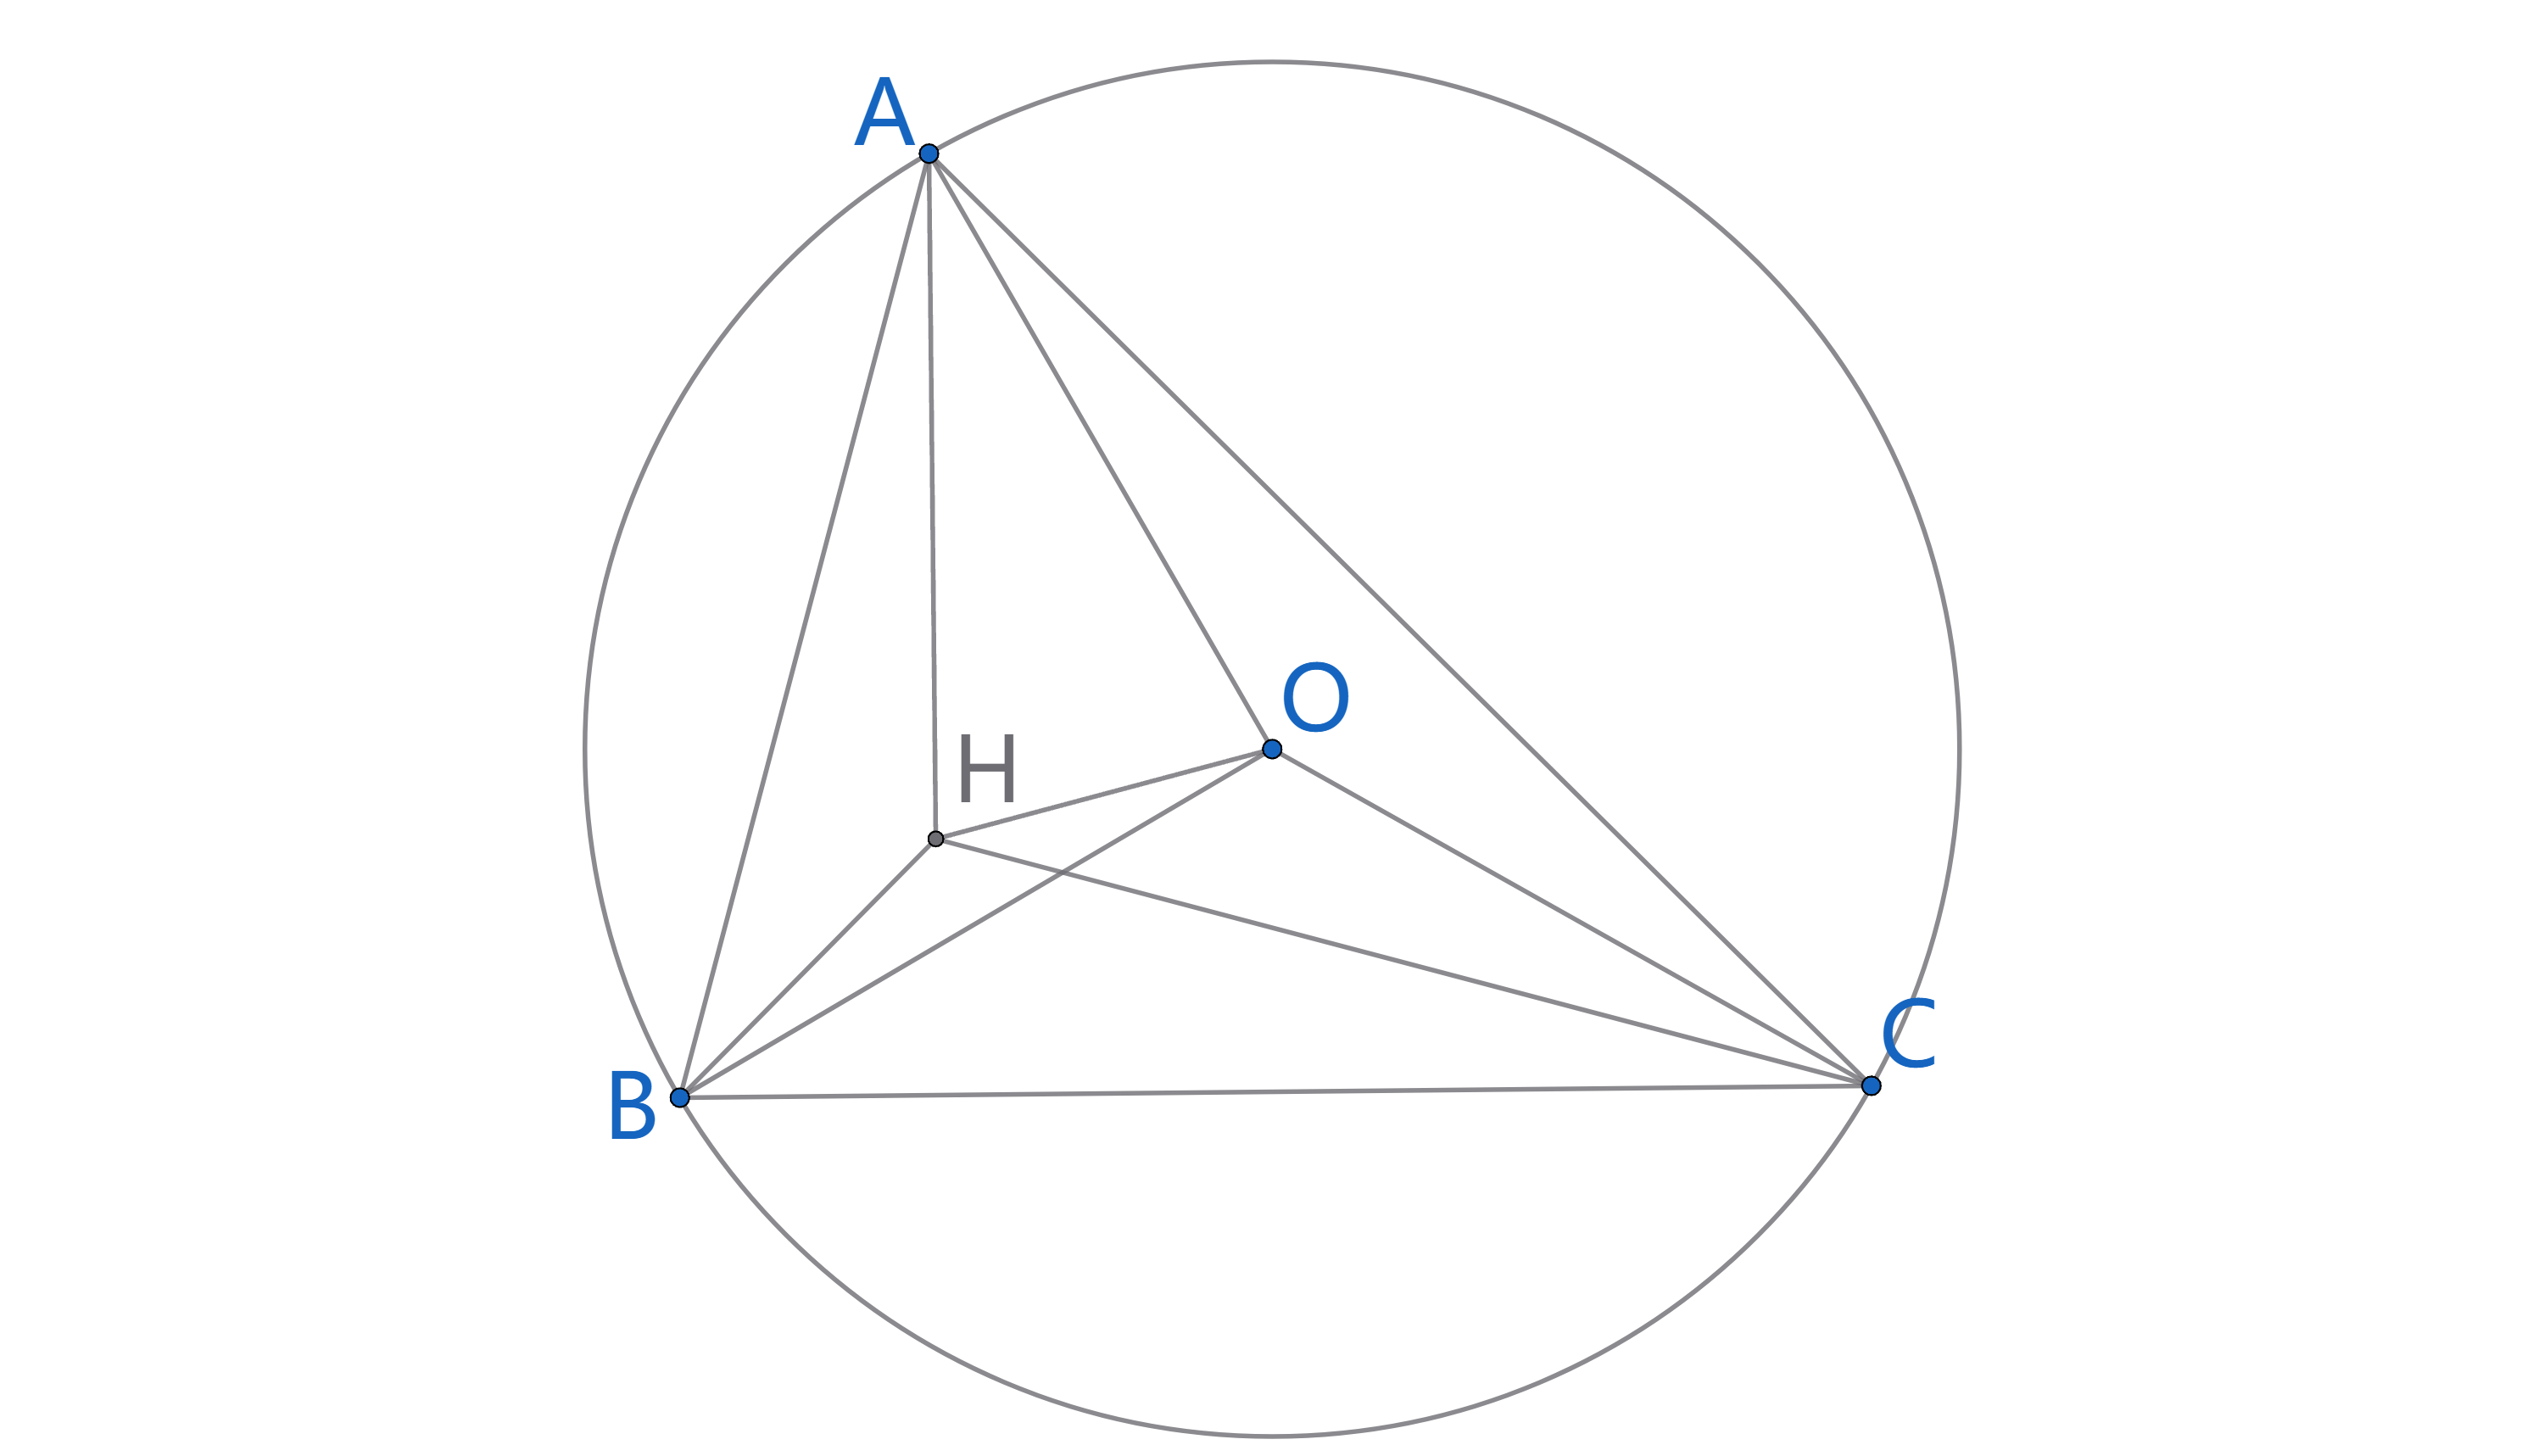
\includegraphics[width=0.7\linewidth]{figures/exercises/327.png}
\end{figure}

% \begin{exercise}
%     (预选题 2001/G1) 给定锐角 $\triangle ABC$,作正方形内接于 $\triangle ABC$,使得正方形的两个顶点在边 $BC$ 上,另外两个顶点分别在边 $AB$ 和 $AC$ 上,这个正方形的中心记为 $A_1$,类似地定义 $B_1, C_1$。证明:直线 $AA_1, BB_1, CC_1$ 共点。
% \end{exercise}
% \begin{figure}[H]
%     \centering
%     \includegraphics[width=0.7\linewidth]{figures/exercises/328.png}
% \end{figure}

%-----------------------------------
\newpage 
\begin{exercise}
    (USATSTST 2011/4) 锐角 $\triangle ABC$ 内接于圆 $\omega$。设 $H$ 和 $O$ 分别表示它的垂心和外心,设 $M, N$ 分别是 $AB, AC$ 的中点。射线 $MH, NH$ 分别与圆 $\omega$ 相交于 $P, Q$,直线 $MN$ 和 $PQ$ 相交于 $R$。证明:$OA \perp AR$。
\end{exercise}
\begin{figure}[H]
    \centering
    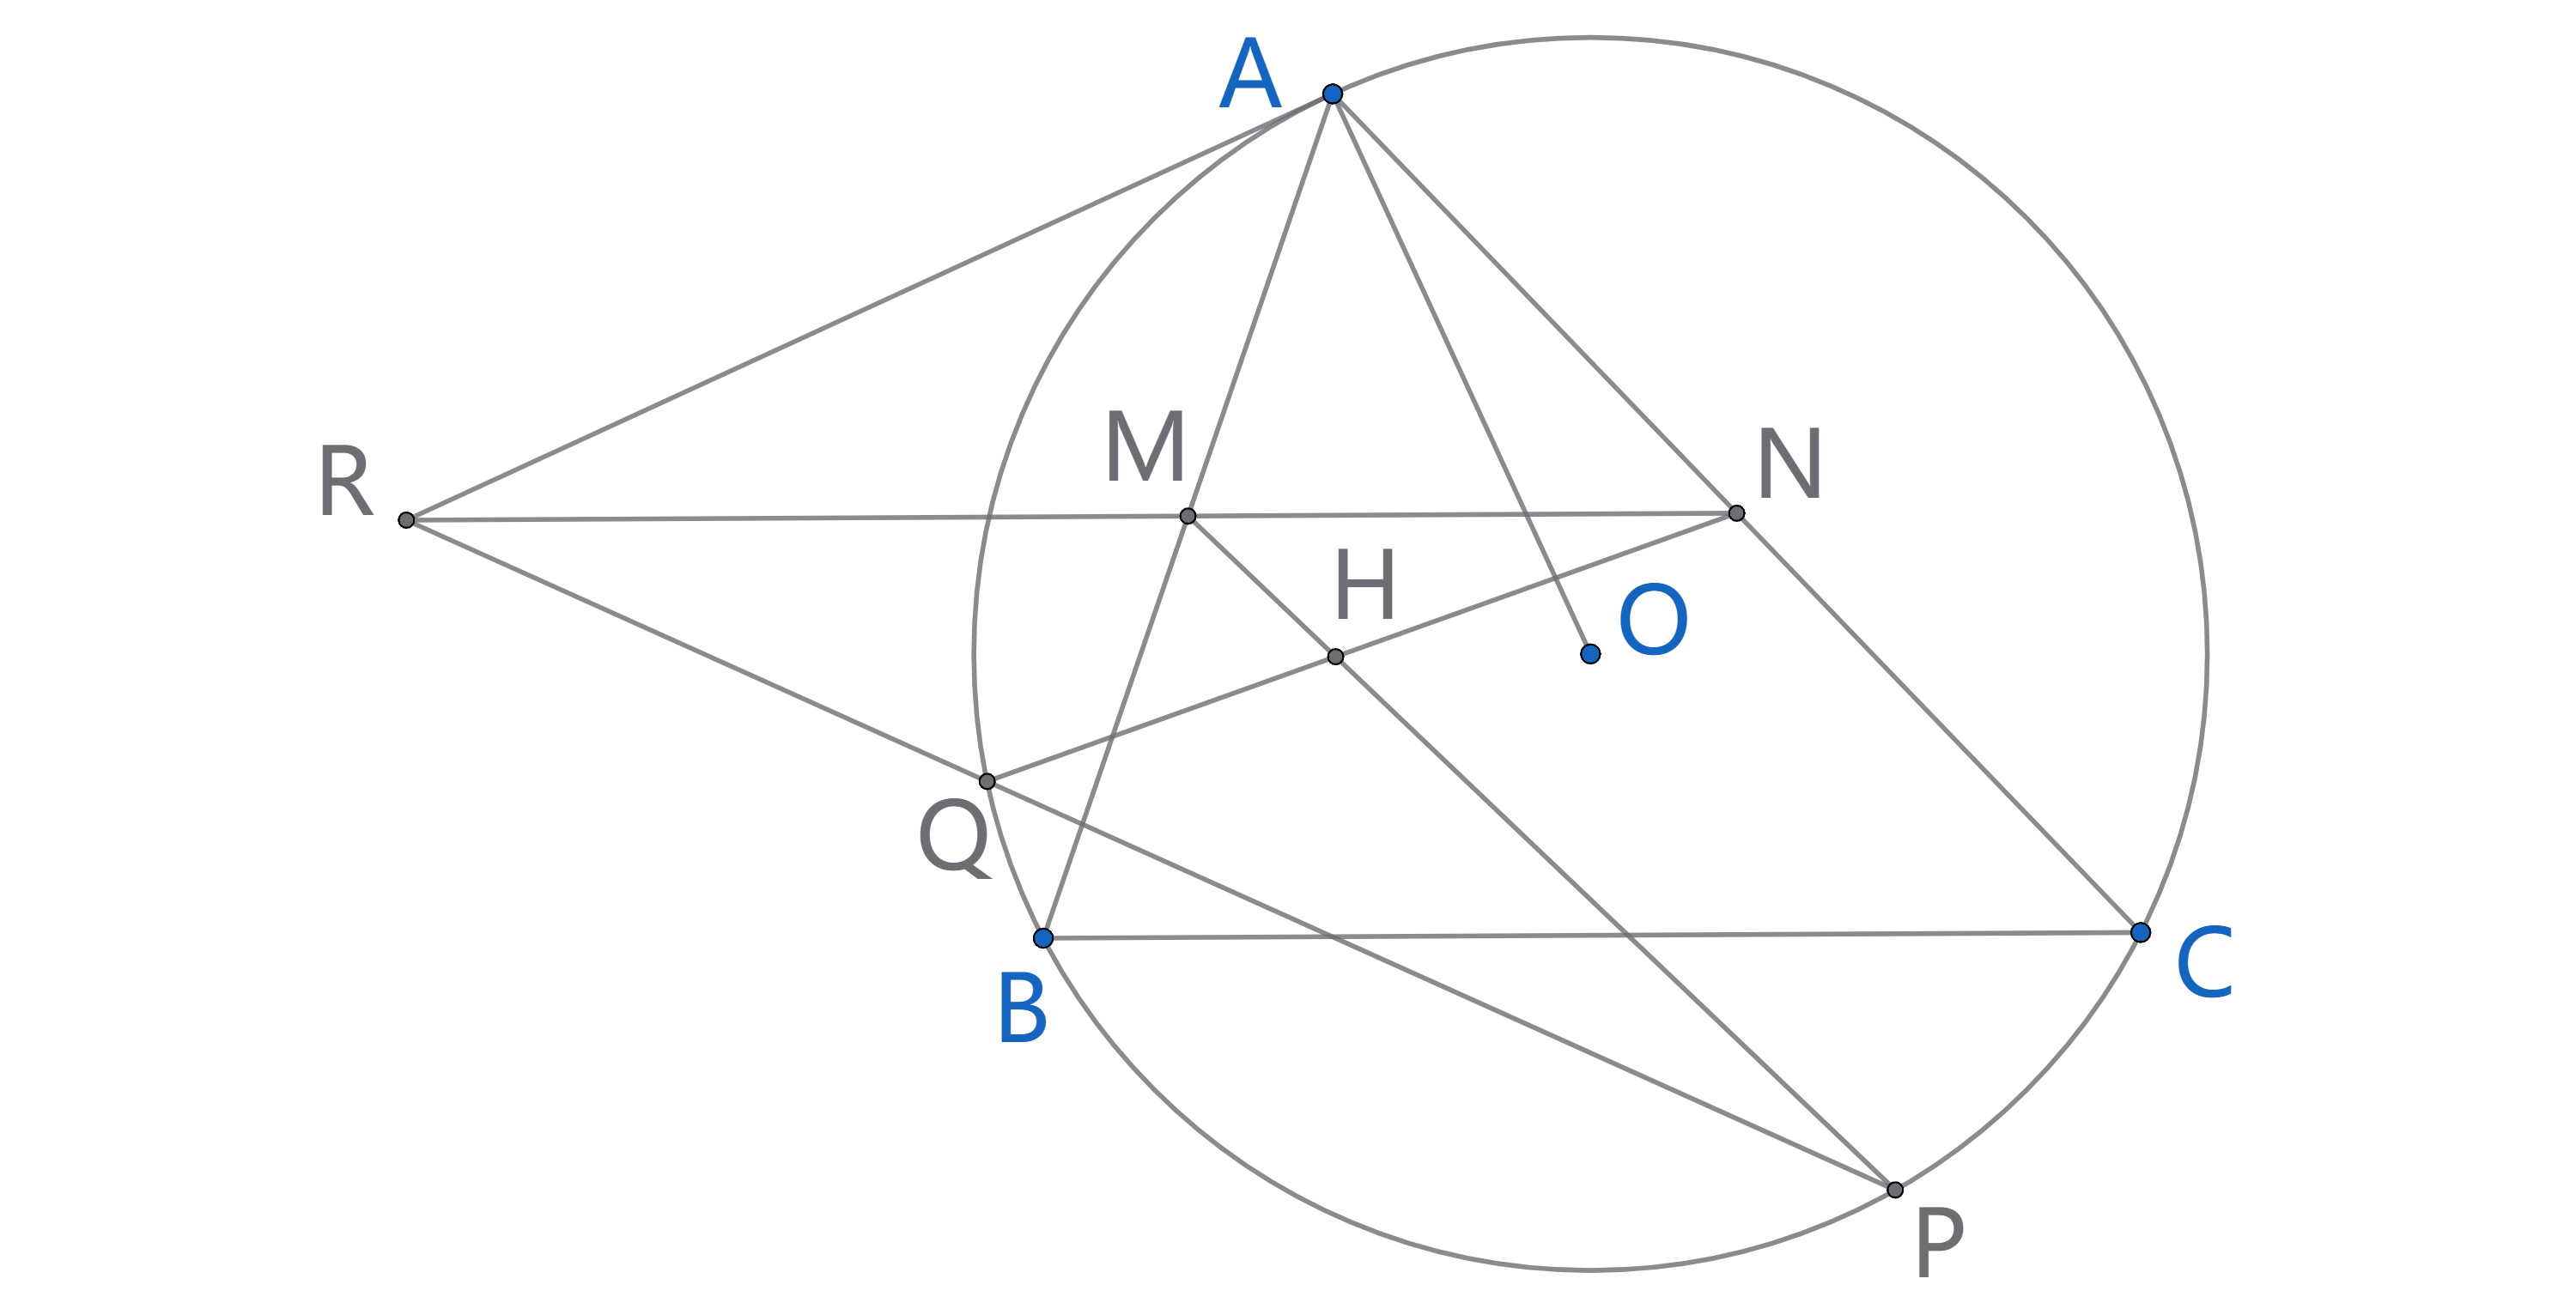
\includegraphics[width=0.7\linewidth]{figures/exercises/329.png}
\end{figure}

\begin{exercise}
    (USAMO 2015/2) 四边形 $APBQ$ 内接于圆 $\omega$,$\angle P = \angle Q = 90^\circ$,$AP = AQ < BP$。设 $X$ 是线段 ${PQ}$ 上的动点。直线 $AX$ 与圆 $\omega$ 相交于不同于 $A$ 的一点 $S$。点 $T$ 在 $\omega$ 的弧 $\overset{\frown}{AQB}$ 上,使得 $XT \perp AX$。设 $M$ 是弦 ${ST}$ 的中点。当 $X$ 在 ${PQ}$ 上变动时,证明:$M$ 在某固定的圆上。
\end{exercise}
\begin{figure}[H]
    \centering
    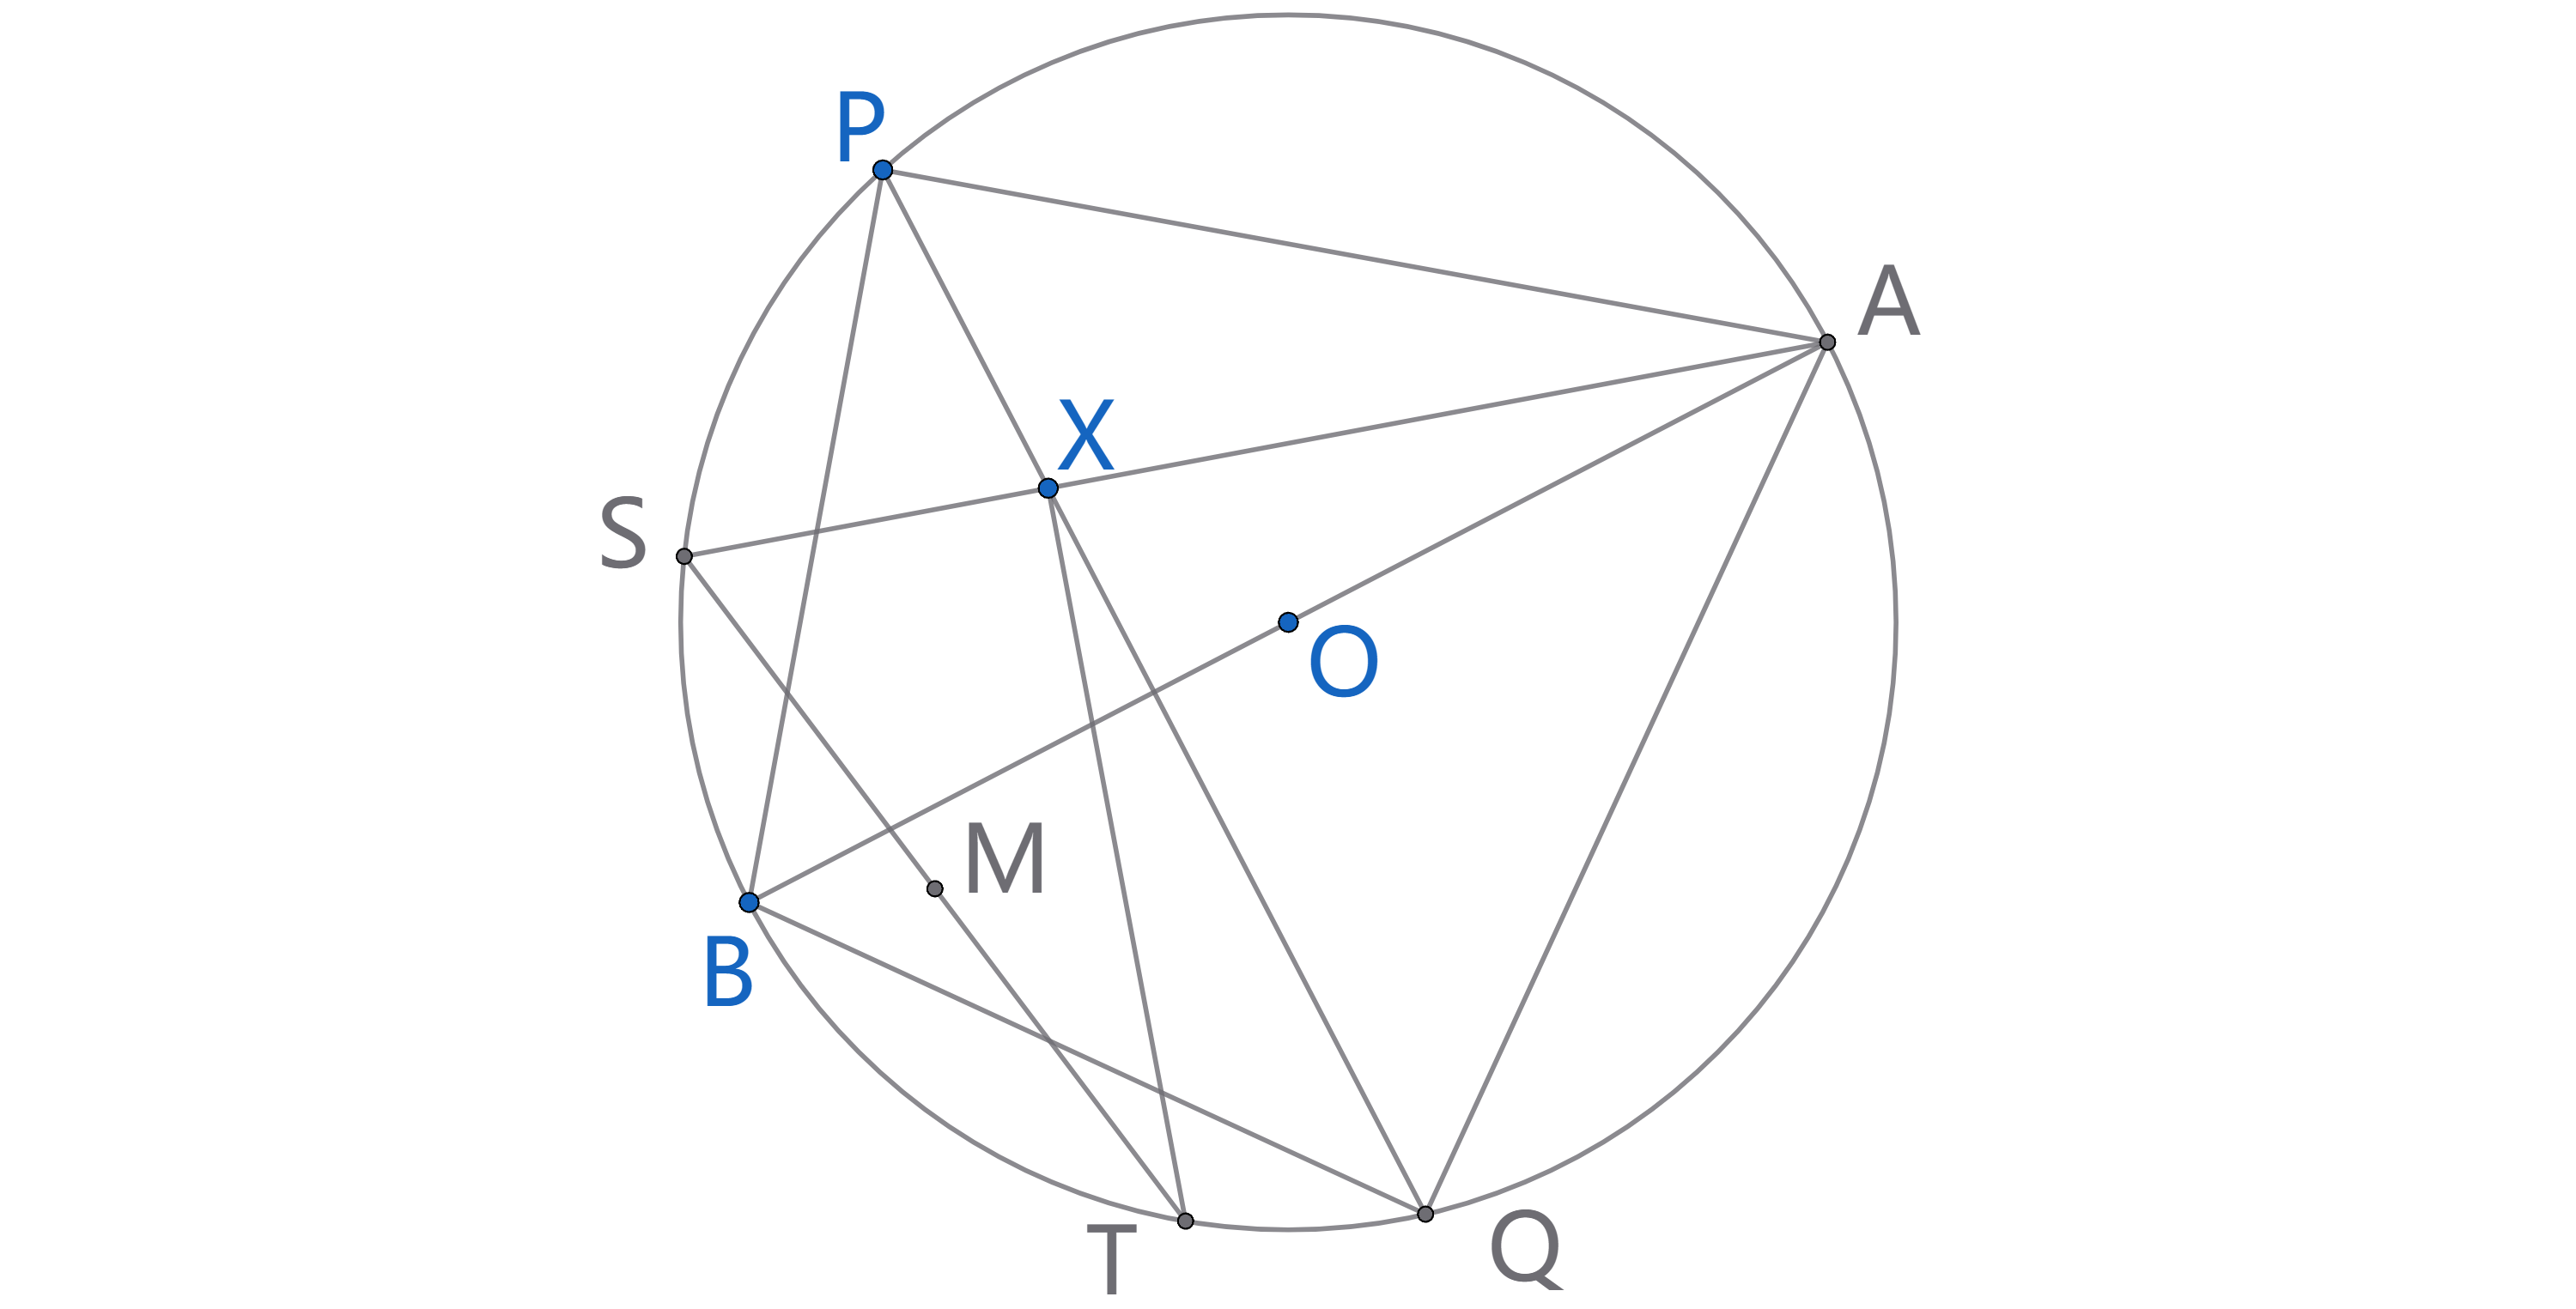
\includegraphics[width=0.7\linewidth]{figures/exercises/330.png}
\end{figure}
